%\vspace{-5pt}
\section{Evaluation}\label{sec:eval}
We now evaluate the computational complexity, localization and mapping accuracy of our Wi-Fi augmented SLAM algorithms. 
Section~\ref{subsec:slam-performance} describes the metrics used for evaluation in detail. 
In section~\ref{subsec:dataset}, we provide information about our setup for data collection and the collected datasets. 
Finally, we describe our results for all the datasets.
%\vspace{-5pt}
\subsection{Metrics to evaluate SLAM performance}
\label{subsec:slam-performance}
%\vspace{\vertspcposthead}
Here are some metrics that indicate SLAM performance: \\
\textbf{False Positive/Negative in Computing Loop Closure}: Identifying incorrect loop closures (false positive) and missing correct ones (false negative), especially in long-term, could have a huge effect on the accuracy of the constructed map. 
Based on ground truth knowledge of our datasets, we count the false positive and false negative loop closures for each SLAM algorithm. 
For this purpose, we find all loop closures that any well-constructed map has detected. Then any extra loop closure is counted as false positive and any missing one is counted as false negative.  \\
\textbf{Error in Estimated Trajectory}: 
%Since the estimated trajectory via SLAM is not necessarily in the same frame as ground truth, we use Kabsch algorithm~\cite{kabsch} for aligning the ground truth path and the estimated trajectory. 
As described below, we record ground truth for our datasets. To measure error, we use the Kabsch algorithm~\cite{kabsch} to align the trajectory generated
by the SLAM algorithm with the ground truth as they are not in the same coordinate frames. 
Then we calculate the RMS error between corresponding poses of ground truth trajectory and estimated trajectories
using the SLAM algorithm. \\
%Then, we calculate the error between the corresponding poses of ground truth trajectory and estimated trajectories using  
%\begin{equation} 
%    E = \frac{1}{N} \sum_{i = 1}^{N} \sqrt{(x_{i}^{(1)} - x_{i}^{(2)})^{2} + (y_{i}^{(1)} - y_{i}^{(2)})^{2}}
%\label{eq:error}
%\end{equation}
\textbf{Computation Time}: A principal challenge for SLAM approaches is the amount of time required to process the data.
 For all three algorithms, we have measured the difference in computation time between the original algorithm and our Wi-Fi augmented version. 
 More specifically, we micro-benchmark the difference in computation times for individual steps from our proposed approach. 
 This includes the reduction in computation time due to {\it Bounding Loop Closure} and the overhead resulting from {\it Wi-Fi Clustering} and {\it Cluster Management}.  
%\vspace{-5pt}
\subsection{Datasets}
\label{subsec:dataset}
Datasets with Wi-Fi measurements alongside RGBD measurements are not readily available. 
Hence, we collected four different datasets from four different buildings at our university.

For data collection, we used a Turtlebot\footnote{\url{https://www.turtlebot.com/turtlebot2/}} mounted with a Kinect 360 and a Velodyne VLP-16 LiDAR~\footnote{\url{http://velodynelidar.com/vlp-16.html}}. 
The Kinect 360 provides RGB-D data with RGB images of 640X480 resolution at 30 frames per second and depth images of 320X240 resolution at 30 frames per second. 
Its depth range goes from 1m to 4m approximately. The LiDAR provides 300,000 points per second with a 360\degree horizontal field of view and $\pm 15$\degree vertical field of view. 
It has a depth range of over 100m. 
In our datasets, the LiDAR is used for ground truth trajectory estimation. 
For this purpose, we used {\it Google Cartographer}~\cite{cartographer} for 2D ground truth trajectory estimation at a 5 cm resolution. %\kar{how much we are doing better? is it higher than this accuracy?}. 
All data is collected using ROS\footnote{\url{http://wiki.ros.org/}} and a laptop on the Turtlebot during execution. We use Intel 7265 wireless card for our Wi-Fi measurements.

We collected four separate datasets from four buildings on campus. \\
%\begin{itemize}
\textbf{C Hall:} This dataset was collected during traversal of a medium-sized square loop with corridors that are 20 meters long. There are 24000 images, less than 40 APs and a total of 7 Wi-Fi clusters in this dataset.\\
\textbf{B Hall:} This dataset includes one long and one short loop that links together to look like the number 8. There are 28000 images, about 40 APs and 13 Wi-Fi clusters in this dataset.\\
\textbf{J Hall:} This dataset includes one long loop and an adjoining trajectory which together looks like the number 9. There are a total of 19 Wi-Fi clusters, around 70 APs and 33000 images in this dataset.\\
\textbf{A Hall:} This dataset is one loop of a long jogging track with sparse visual features. There are not many blocking walls between different places on the trajectory. The number of frames, APs and Wi-Fi clusters are 50000, 45 and 8 respectively.
%\end{itemize}
%\subsubsection*{Statistics}
%\zaki{provide a table of number of clusters and frames of datasets in order to give some explanations about how number of clusters are affected.} 
%\vspace{-5pt}
\subsection{RGBD SLAM performance}
As we ran the RGBD SLAM with default parameter settings on {\it C Hall} dataset, we got very inaccurate maps and trajectories. 
So, we decided to perform parameter tuning and find the best possible outcomes of vanilla RGBD SLAM based on our metrics defined above. 
%The parameters are {\it min-matches} and {\it inlier-distance}.
The first parameter is the minimum number of matched features required for accepting a transformation which is called {\it min-matches}.
The second parameter is the maximum distance allowed for inlier points when using RANSAC for transformation estimation and is called {\it inlier-distance}.

%Increasing min-matches decreases the possibility of matches and has the effect of reducing false positives and increasing false negatives. 
%Increasing inlier-distance has the effect of increasing false positives and decreasing false negatives. 
We pick three different reasonable values for inlier-distance and four values for min-matches and run vanilla RGBD SLAM on each set of parameters for {\it C Hall Dataset}. 
\begin{figure*}
	\begin{subfigure}[b]{.3\textwidth}
		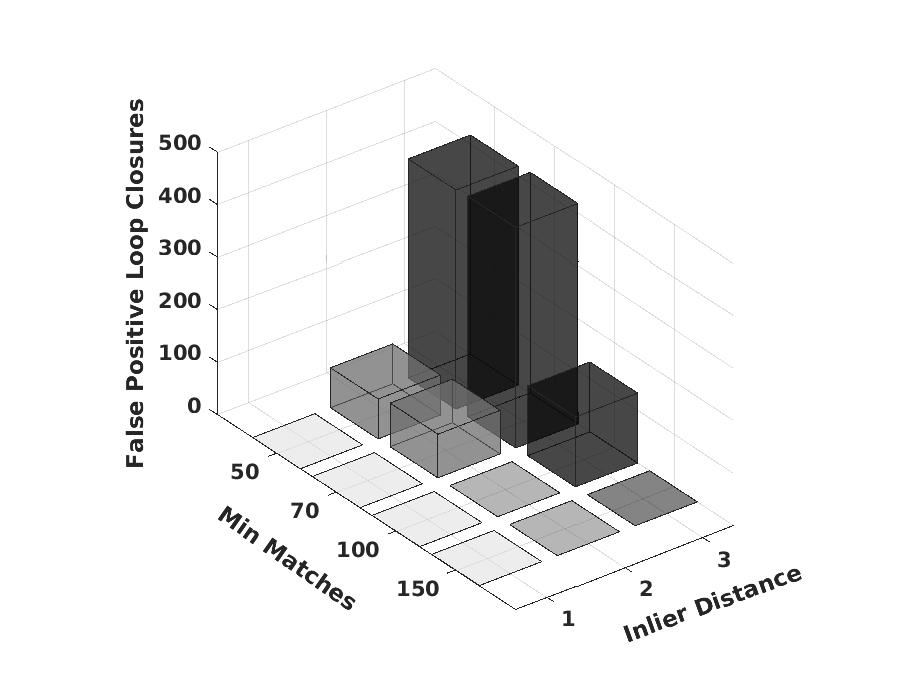
\includegraphics[width=\textwidth]{Figure6_a.eps}
		%\label{subfig:center}
		%\vspace{-6mm}
		%\caption{Number of false loop closures}
	\end{subfigure}
	\begin{subfigure}[b]{0.3\textwidth}
		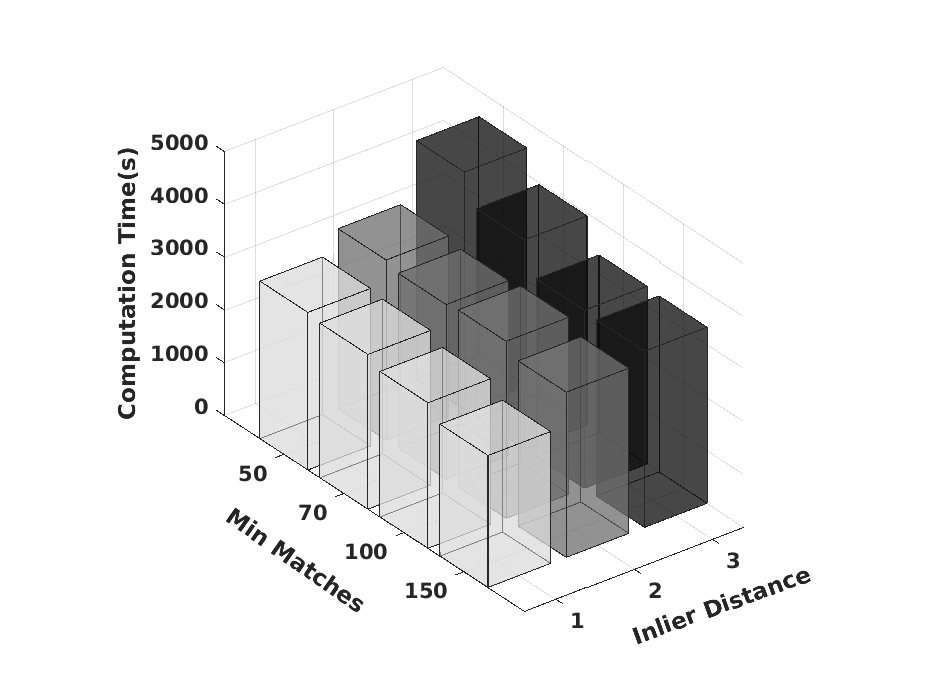
\includegraphics[width=\textwidth]{Figure6_b.eps}
		%\label{subfig:center}
		%\vspace{-6mm}
		%\caption{Number of keyframes}
	\end{subfigure}
	\begin{subfigure}[b]{0.3\textwidth}
		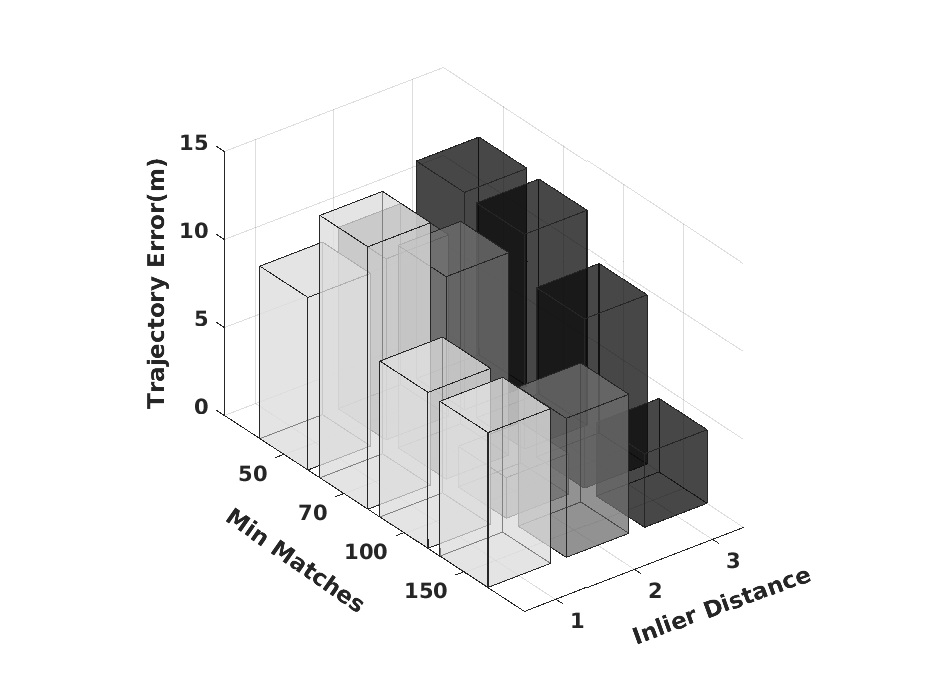
\includegraphics[width=\textwidth]{Figure6_c.eps}
		%\label{subfig:center}
		%\vspace{-6mm}
		%\caption{Estimated Trajectory Error}
	\end{subfigure}
\caption{False positive loop closures (left), computation time (center) and trajectory error (right) when the parameters {\it min-matches} and {\it inlier-distance} are varied. }
\label{RGBD_analysis}
%\vspace{-10pt}
\end{figure*}

%Figure~\ref{RGBD_analysis} shows the behavior of RGBD SLAM algorithm when two parameters are changing.
%One of these parameters is the minimum number of matched features required for accepting a transformation which is called \textit{min matches}.
%The other parameter is the maximum distance allowed for inlier points when using RANSAC for transformation estimation and is called \textit{inlier distance}.

%As it is expected, when \textit{min matches} increases, the number of keyframes increase as well.
%The reason is behind keyframe definition which states if a frame could not be related to any previous keyframe or any frame earlier than the last keyframe, it is a keyframe itself.
%On the other hand, increasing \textit{inlier distance} leads to decrement in the number of keyframes, because the probability of finding a transformation among two frames is higher.
%As observed in the leftmost plots, increasing \textit{min matches} and decreasing \textit{inlier distance}, usually decreases the number of false positive loop closures.
%Because increasing the \textit{min match} parameter makes it harder for the algorithm to find transformations having required number of matches among frames.
%In other words, it is less probable to find required number of matches within allowable inlier distance among two distant frames.

From Figure~\ref{RGBD_analysis}, increasing min-matches and decreasing inlier-distance decreases the number of false positives as expected. 
The computation time decreases as the number of min-matches increase and inlier-distance decreases. This is a direct result of the reduction in permissible transformations between frames.
There is a lack of structure in the way trajectory error varies with these parameters. 
Our conjecture is that this is because of the randomness in node selection as well as the effect of associated false positive/negative loop closures. 
%Note that the vanilla RGBD SLAM fails to perform the final loop closure (false negative) for all runs. 

\begin{figure}
\centering
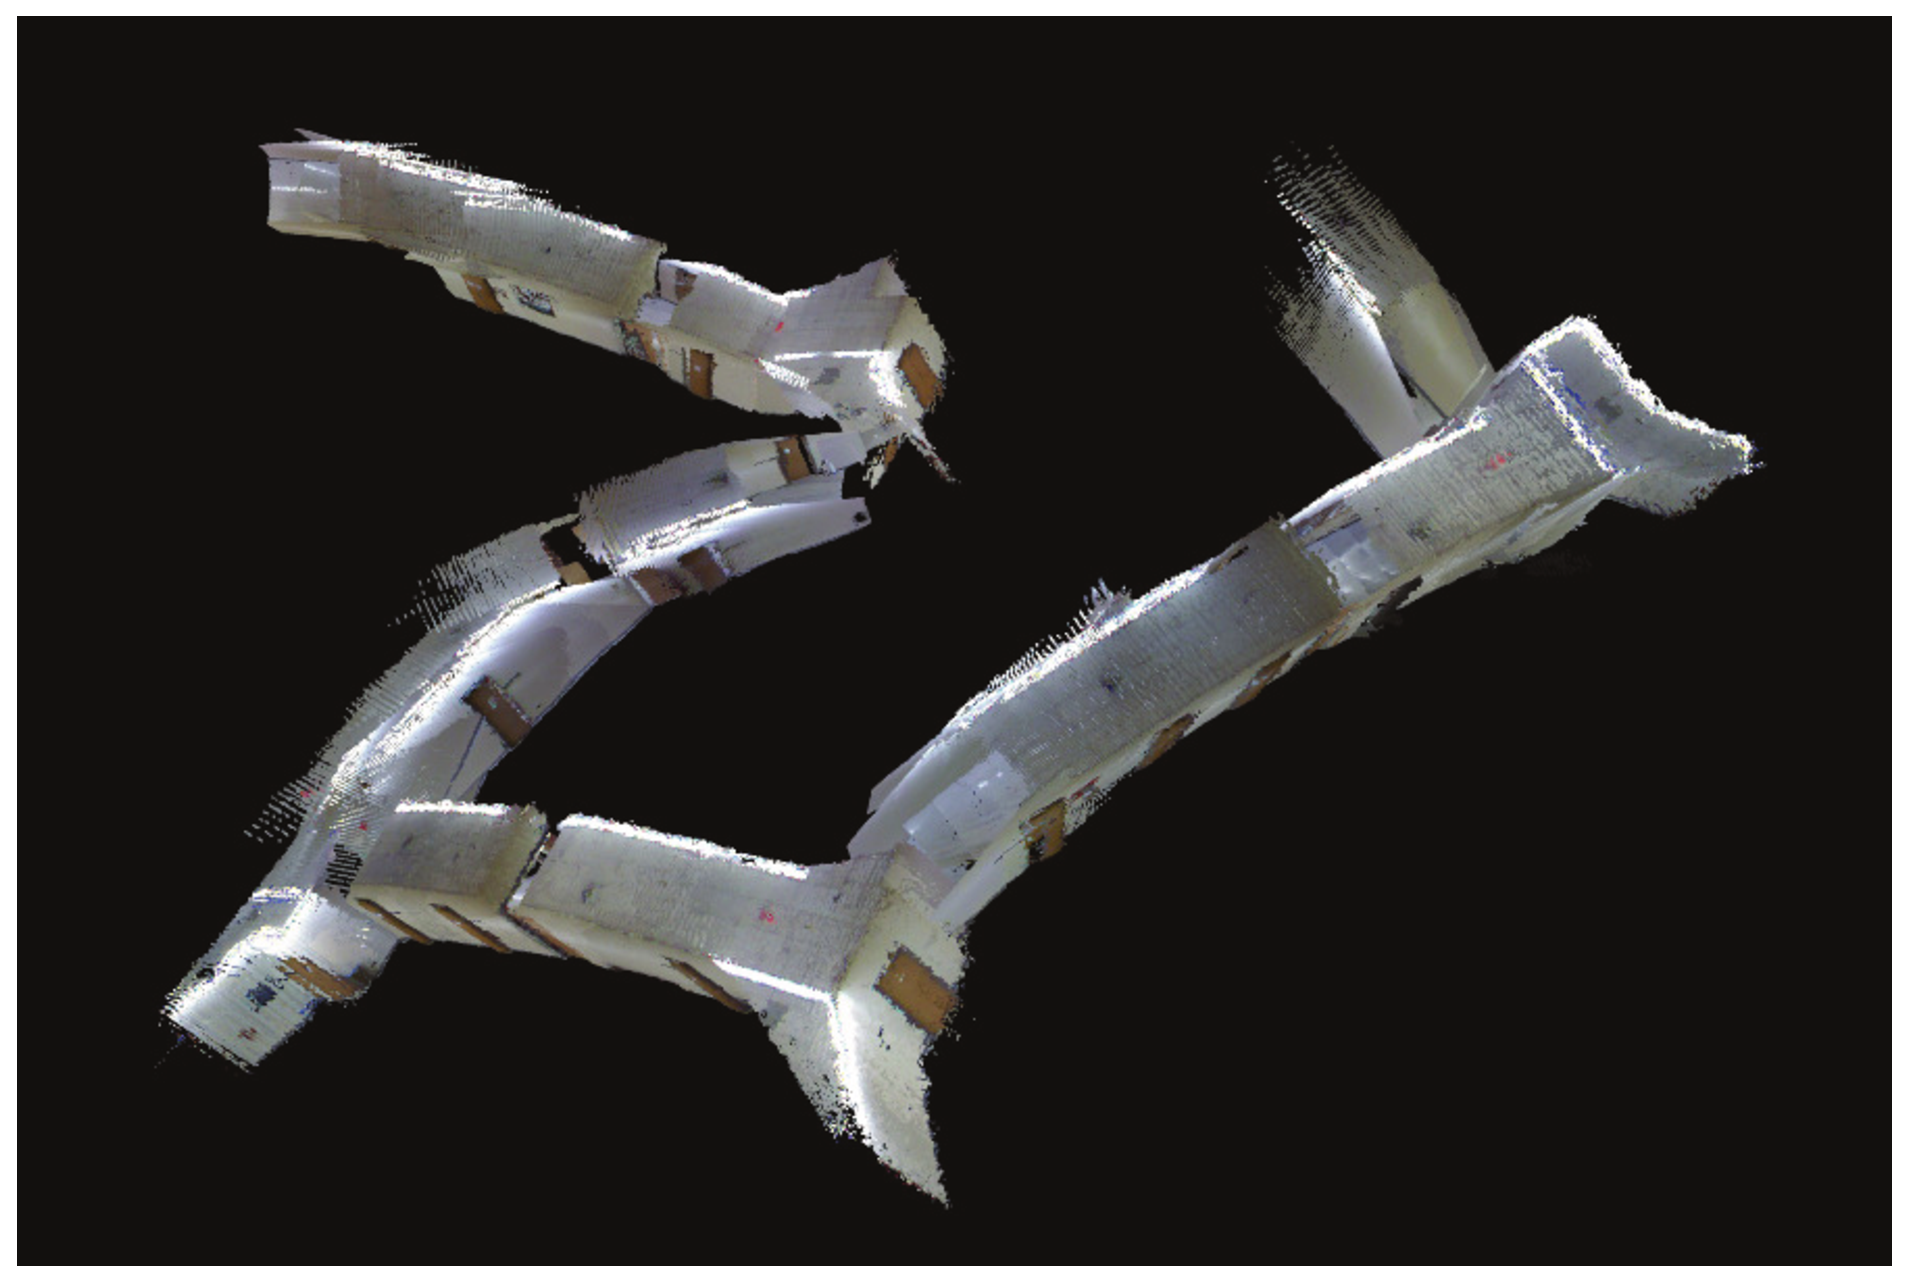
\includegraphics[width=0.2\textwidth]{Figure7_a.eps}
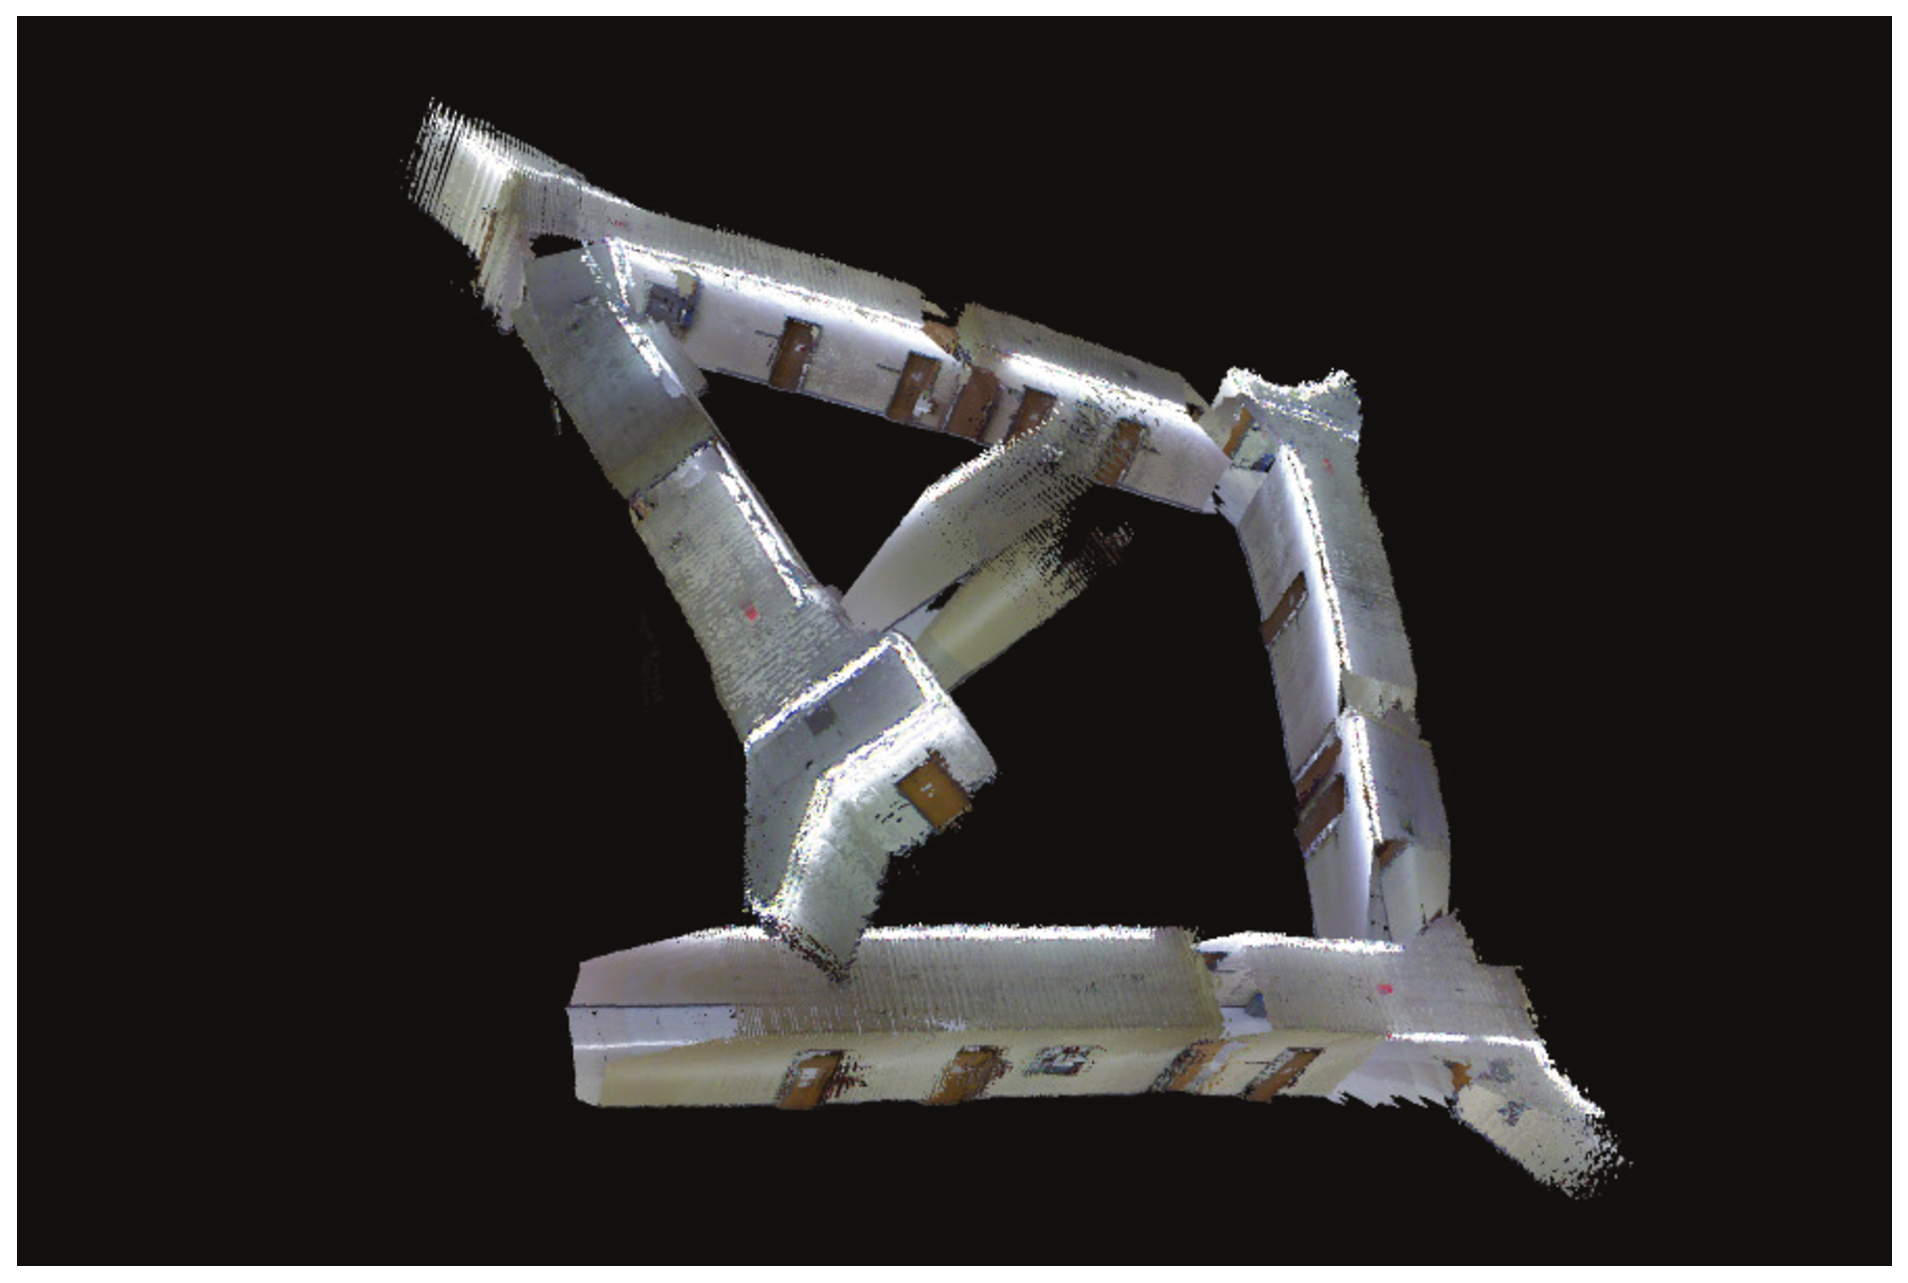
\includegraphics[width=0.2\textwidth]{Figure7_b.eps}
\caption{Constructed maps of vanilla RGBD SLAM with {\it min-match}=100/150 and {\it inlier-distance}=2. Both suffer from rotational deviations due to low number of visual transformations}
\label{fig:rgbd_badmap}
\end{figure}
\vspace{-10pt}
Setting {min-match} to very high values and {inlier-distance} to very low values cause the graph to have a very low number of permissible visual transformations. 
Potentially too low to even create a reasonable map. 
Figure~\ref{fig:rgbd_badmap} shows the constructed maps with {min-match} = 100/150 and {inlier-distance}=2 which suffer from rotational deviations due to a very low number of visual transformations. 
Therefore, we have picked lower values for {min-match} and higher values for {inlier-distance} to provide parameters that give reasonable performance with respect to the number of visual transformations. 
Because Wi-Fi sensing is not able to force a visual transformation if it is rejected due to a very high value of {min-match} or very low value of {inlier-distance}.
%Figure~\ref{fig:RGBDW_maps} represents the two best constructed maps of our proposed method.
%As it is obvious, Wi-Fi incorporation is not only helping in getting rid of many false loop closures, but aids in detecting the final loop closure by making comparisons to related keyframes in close-by regions instead of non-sense random selection.
%It should be noted that the reason behind not very carefully aligned aisles at last loop closure is the way RGBD SLAM calculates visual transformations and doesn't relate to our method.
%However, it should be noted that for settings with very low number of false loop closures, the accuracy of estimated map is almost the same for both original and proposed approach.
%Because even our proposed method could not detect the last loop closure due to very low number of inliers in a feature-less environment.
%But our computation time is lower due to rejection of many transformations due to Wi-Fi dissimilarity among their corresponding frames prior to any effort for visual transformation.

\begin{figure*}
	\begin{subfigure}[b]{.3\textwidth}
		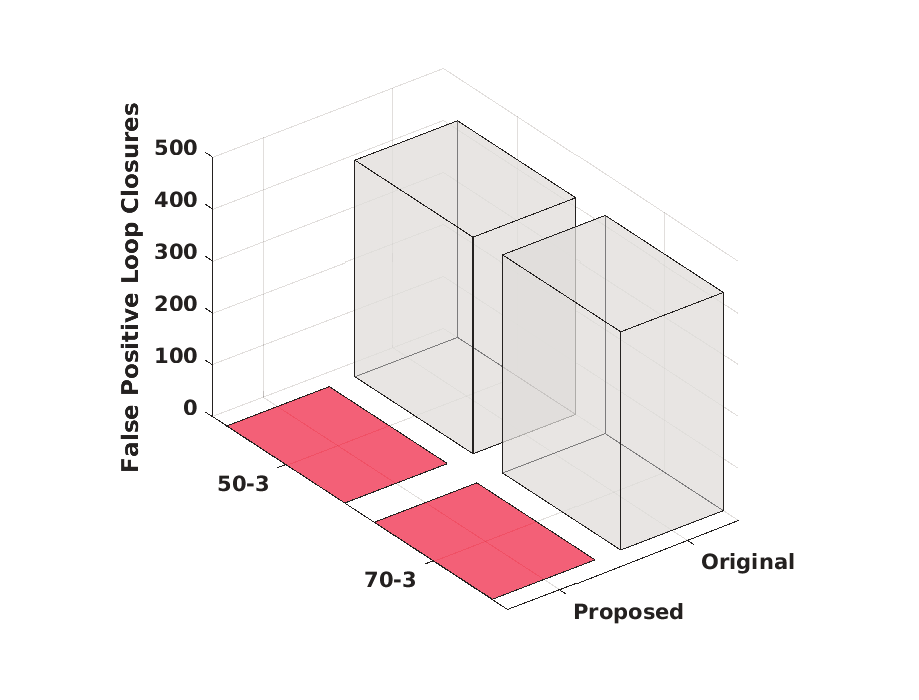
\includegraphics[width=\textwidth]{Figure8_a.eps}
		%\label{subfig:center}
		%\vspace{-6mm}
		%\caption{Number of false loop closures}
	\end{subfigure}
	\begin{subfigure}[b]{0.3\textwidth}
		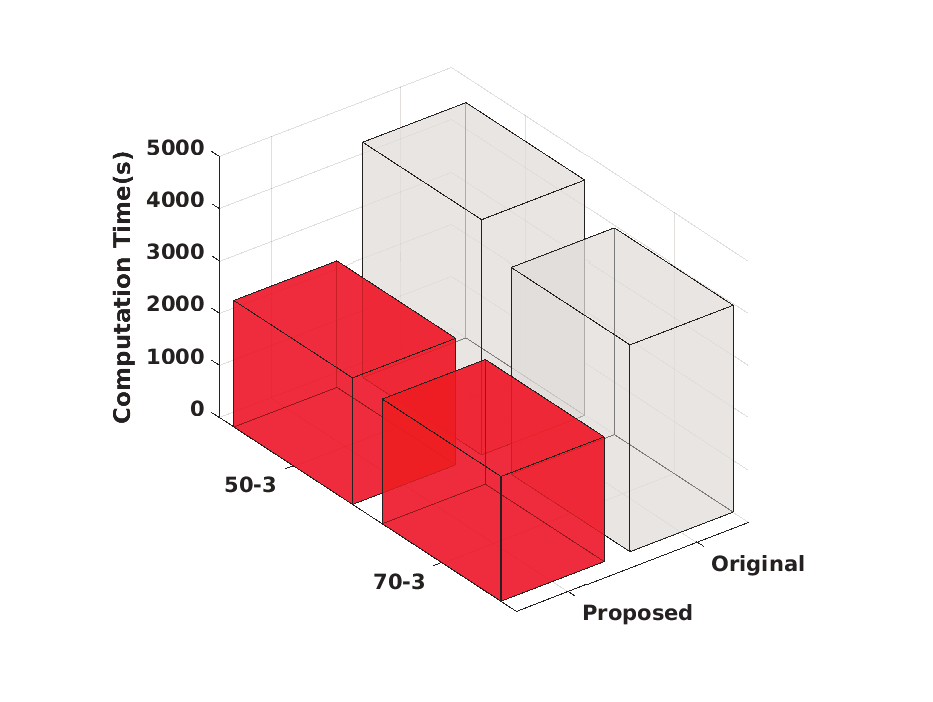
\includegraphics[width=\textwidth]{Figure8_b.eps}
		%\label{subfig:center}
		%\vspace{-6mm}
		%\caption{Estimated Trajectory Error}
	\end{subfigure}
%	\hspace{4mm}
	\begin{subfigure}[b]{0.3\textwidth}
		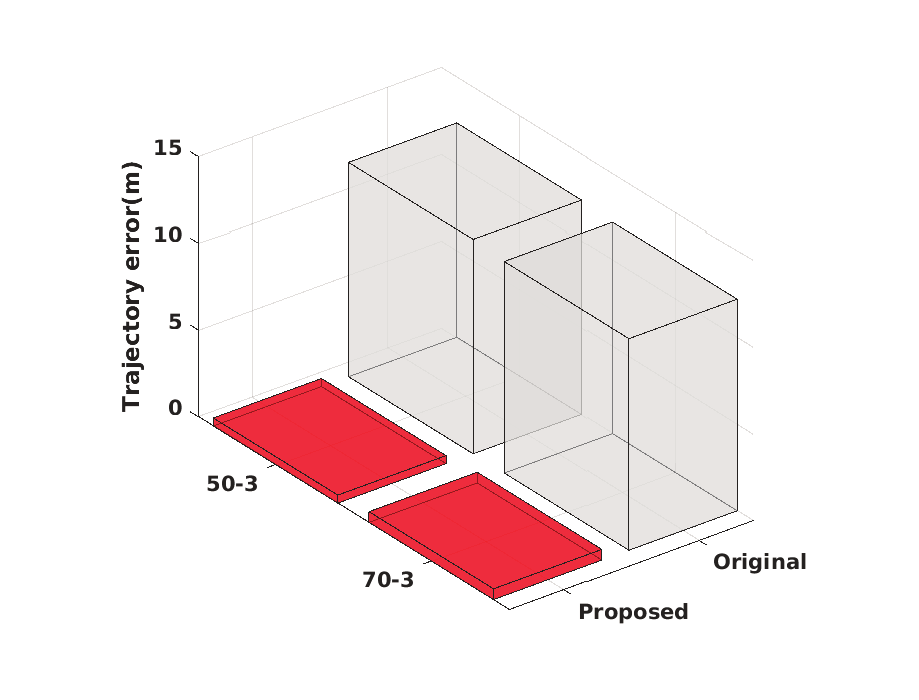
\includegraphics[width=\textwidth]{Figure8_c.eps}
		%\label{subfig:center}
		%\vspace{-6mm}
		%\caption{Number of keyframes}
	\end{subfigure}
%\vspace{-20pt}
\caption{Accuracy comparison between vanilla RGBD SLAM and our proposed method.}
\label{fig:RGBDW_comparison}
%\vspace{\vertspcpostimg}
%\vspace{-20pt}
\end{figure*}
Figure~\ref{fig:RGBDW_comparison} compares the original method and our proposed method for the C Hall dataset.
Results show that our proposed method gets rid of all false loop closures for both settings.%by more than $90\%$ for $min-matches=50$ and more than $80\%$ for $min-matches=70$.
We believe this is because Wi-Fi similarity allows us to identify a good sub-set of keyframes to compare against for accurate loop closure as opposed to the fixed set of random keyframes selected by vanilla RGBD SLAM. 
Similarly, we reduce the computation time of affected modules by {bounding loop closure} by more than $50\%$ for {min-match}=50 and more than $30\%$ for {min-match}=70. 
This is because Wi-Fi similarity allows us to eliminate unnecessary comparisons. 
Moreover, having a smoother map reduces the optimization time as well. 
Finally, we also observe a reduction in RMS error of $80\%$ for min-matches $\in (50, 70)$. 
This is also a result of identifying a good sub-set of keyframes for loop closure comparison and not allowing visual transformations between frames having distant Wi-Fi signatures. 

Based on the shown result, it seems that the performance of RGBD SLAM in symmetric environments with a low number of features is very poor. 
So we decided not to continue running this algorithm on longer and harder datasets in order to avoid unreasonable comparisons.  
%\vspace{-5pt}
\subsection{RTAB-Map performance}
%One main difference between RTABMap and RGBD SLAM is the real time constraint provided in RTABMap.

\begin{figure}[h]
    \centering
    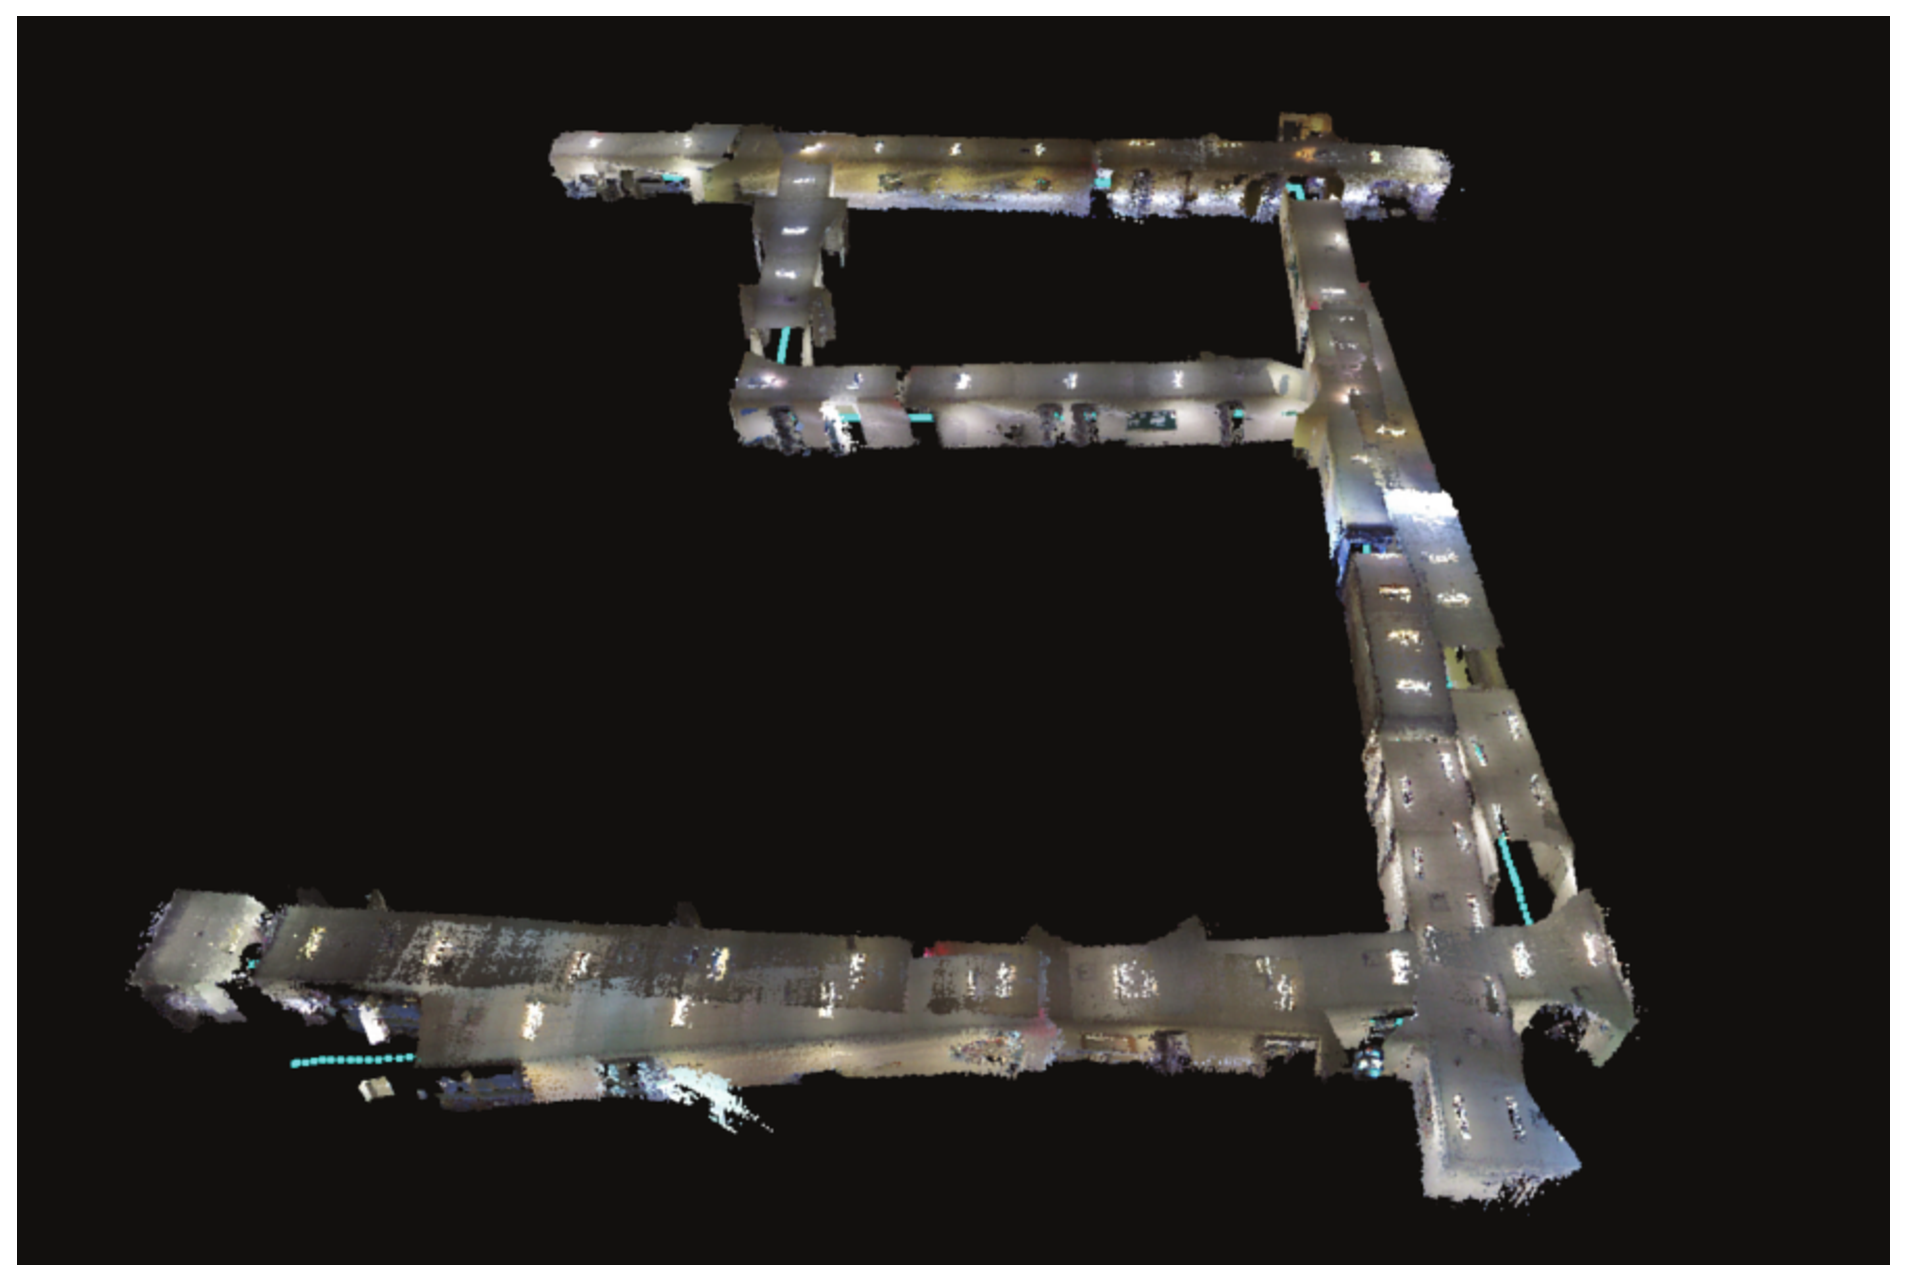
\includegraphics[height=1.0in]{Figure9_a.eps}
    \hspace{.2in}
    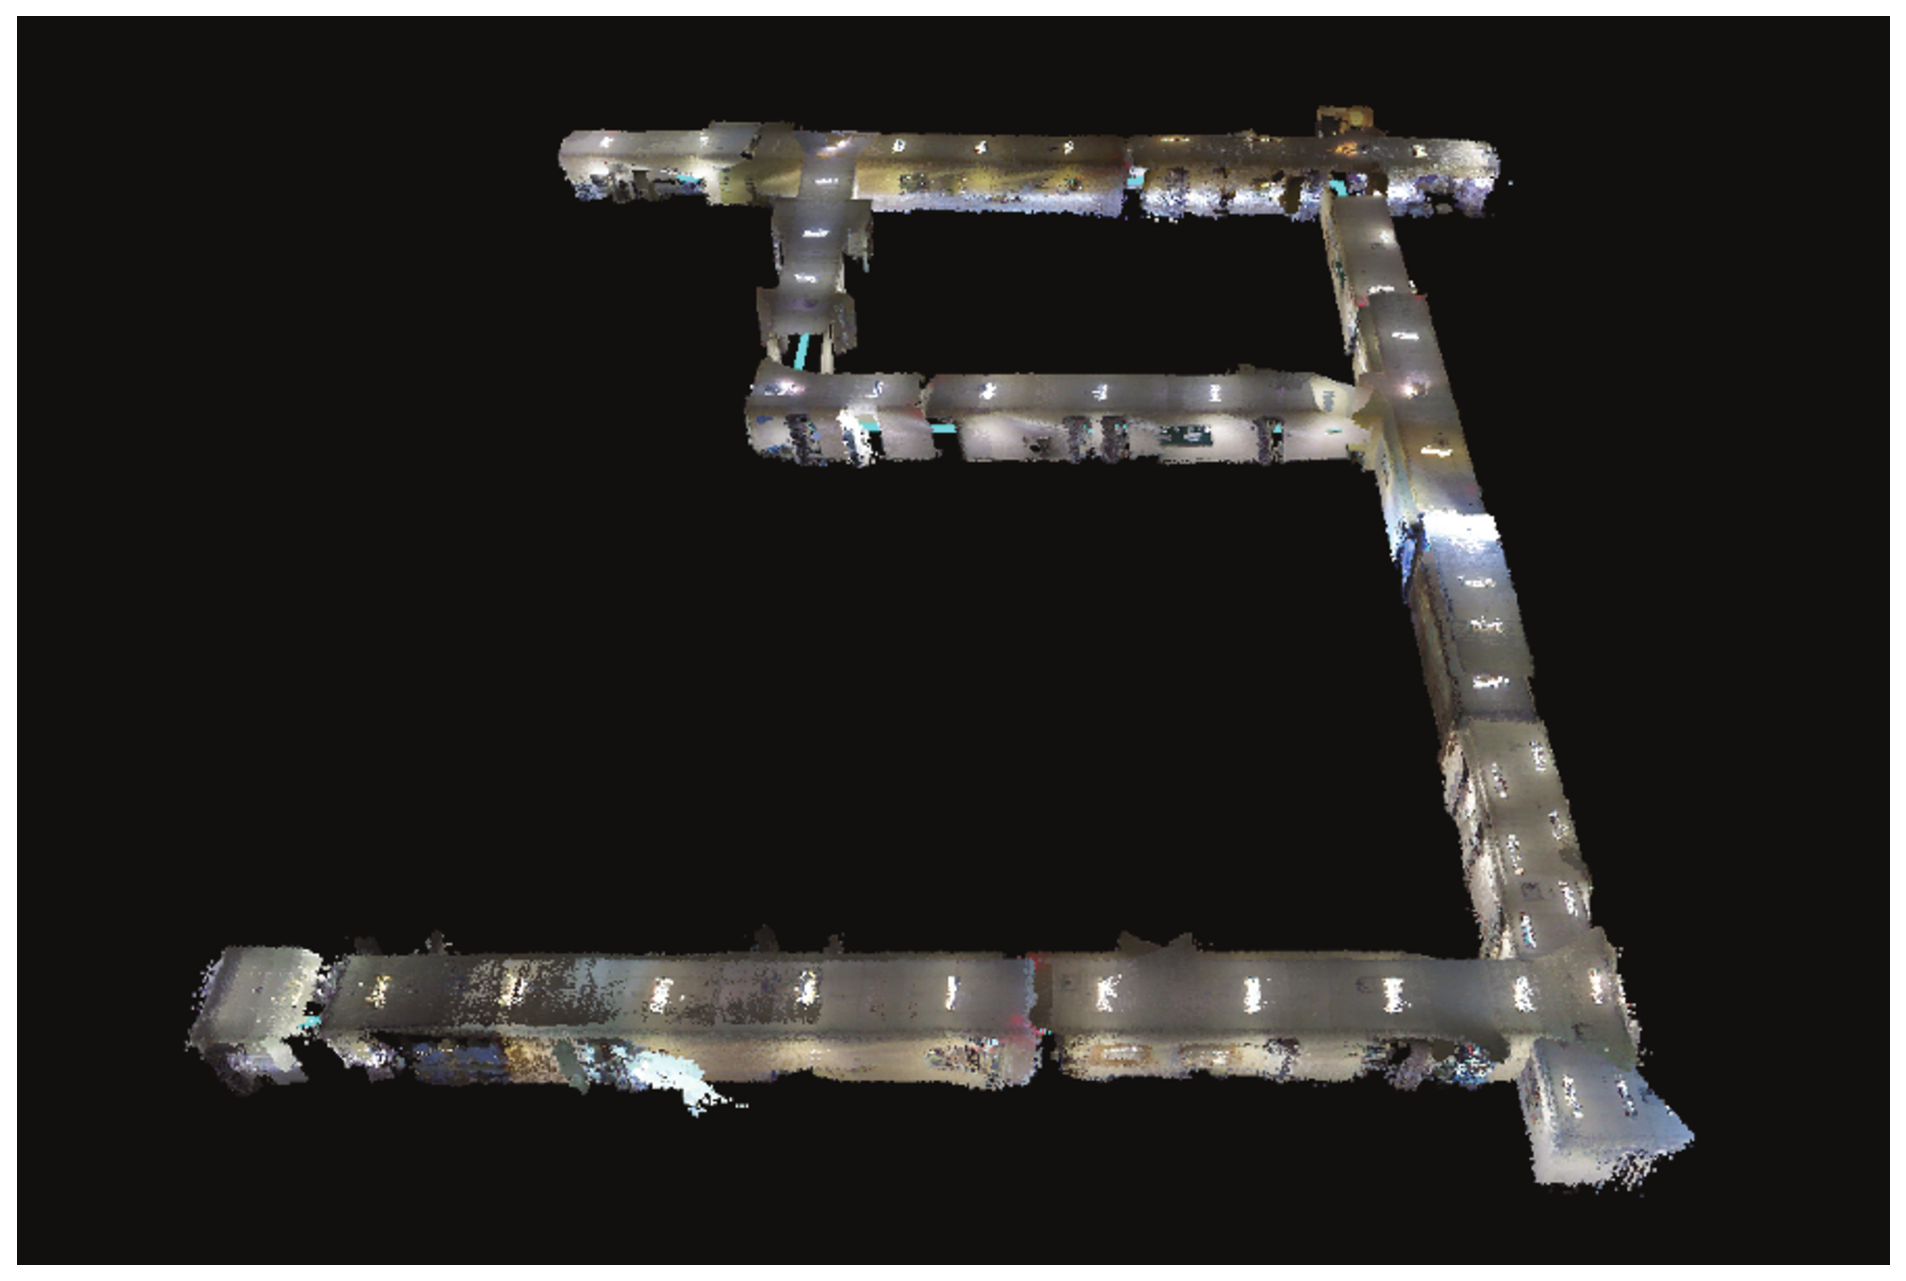
\includegraphics[height=1.0in]{Figure9_b.eps}
    \hspace{.2in}
    %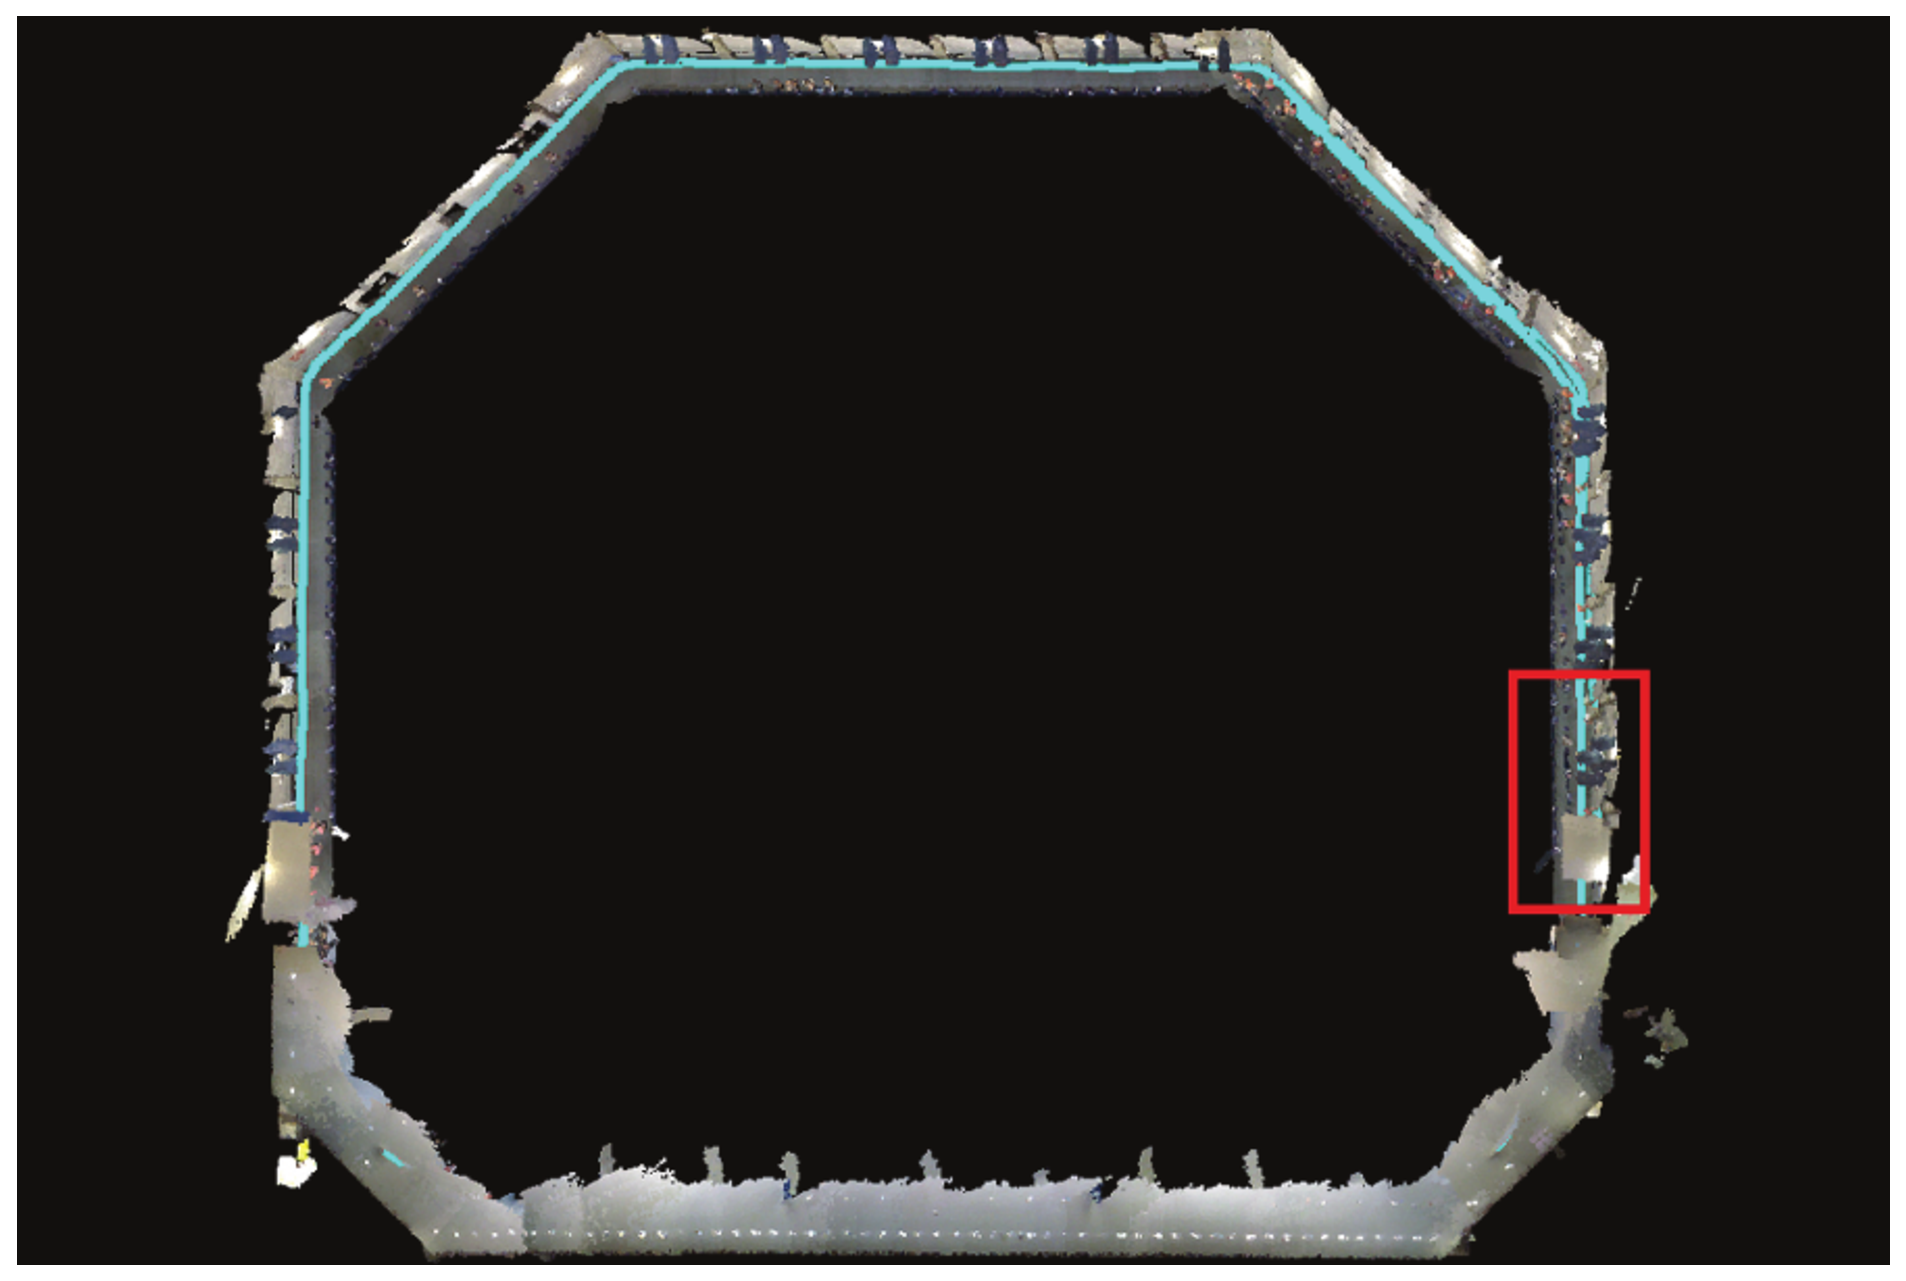
\includegraphics[height=1.0in]{Figure9_c.eps}
    %\hspace{.2in}
    %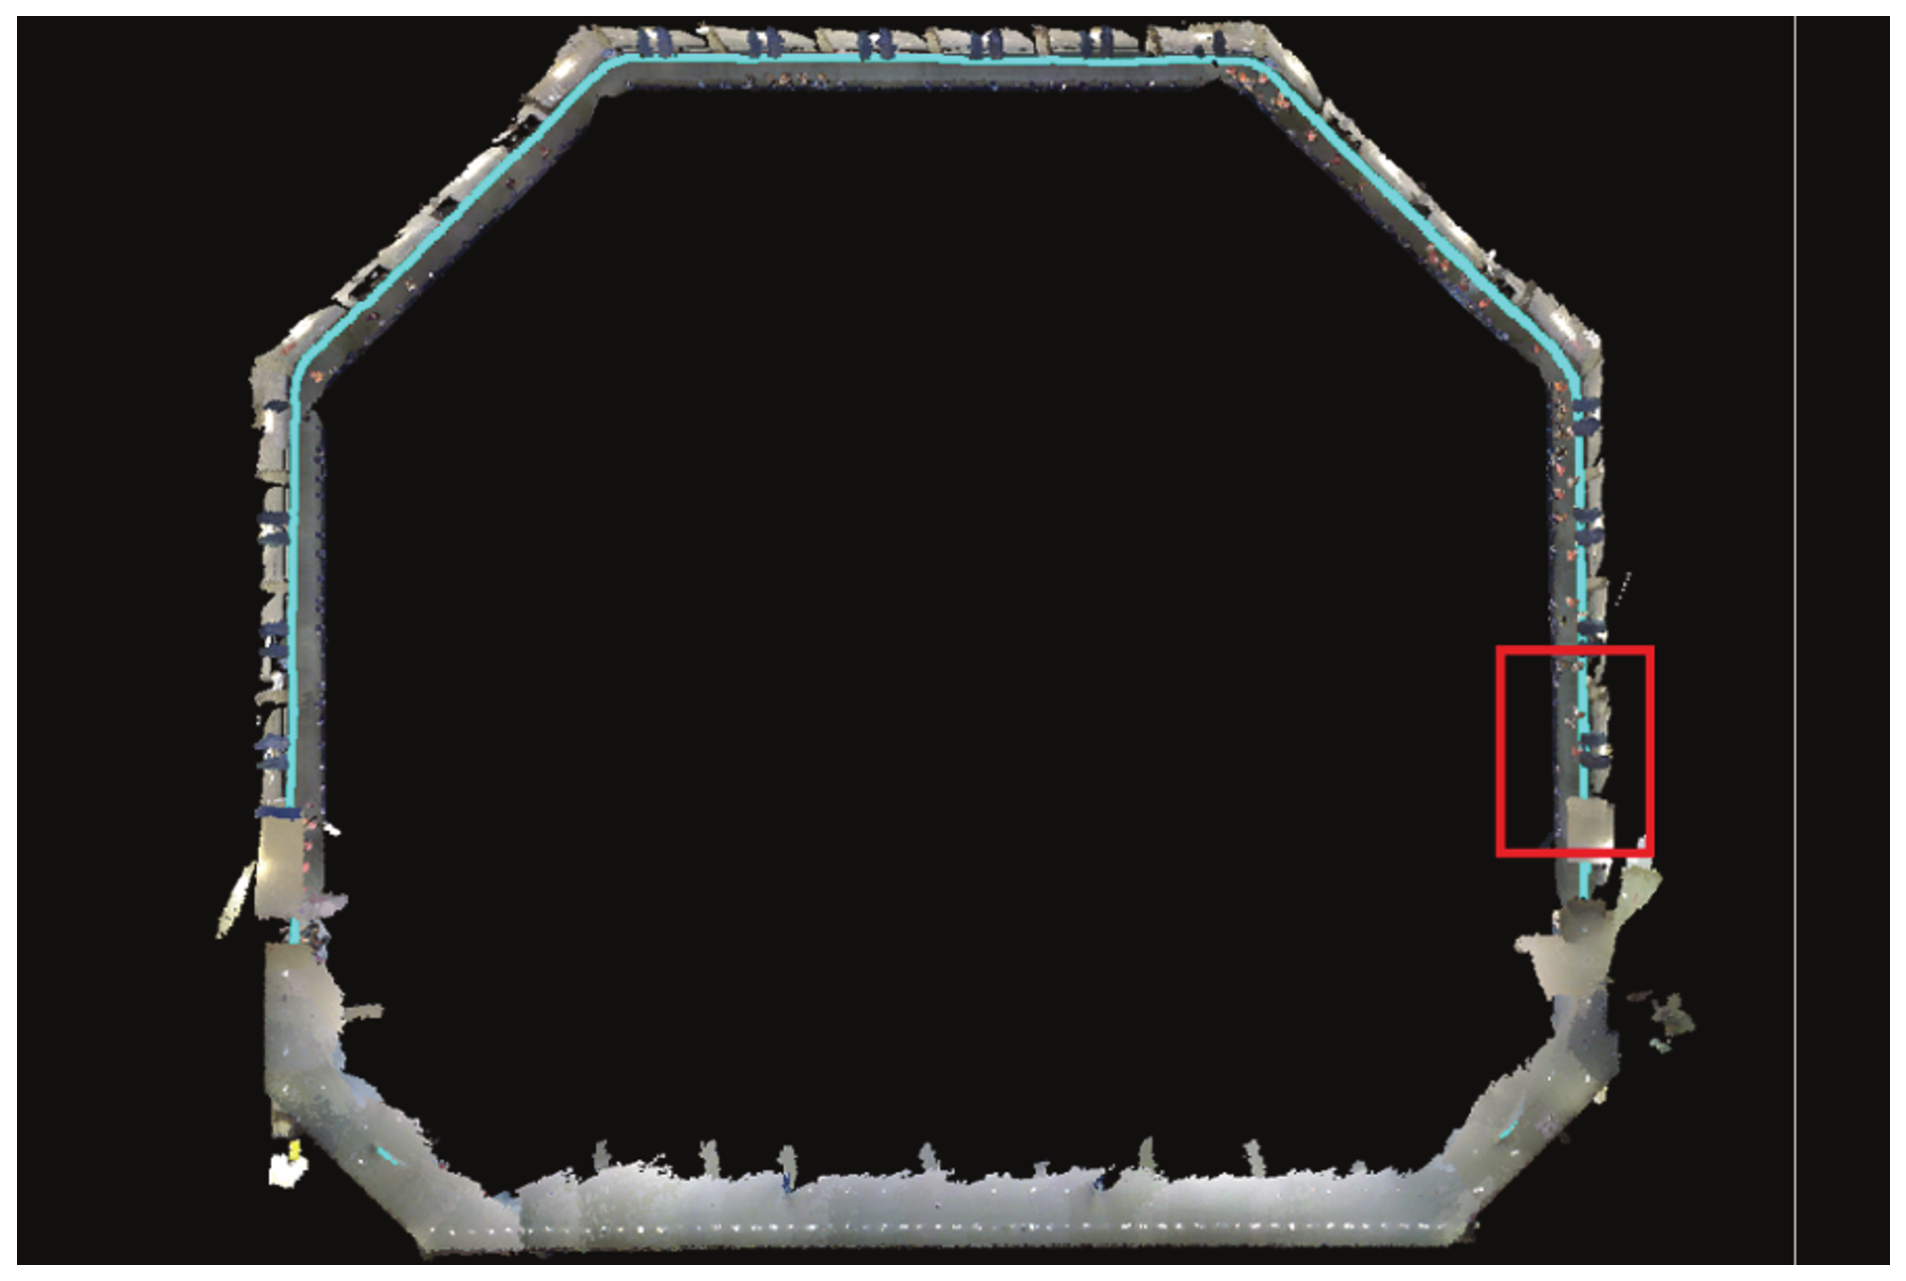
\includegraphics[height=1.0in]{Figure9_d.eps}
    %\hspace{.2in}
   % 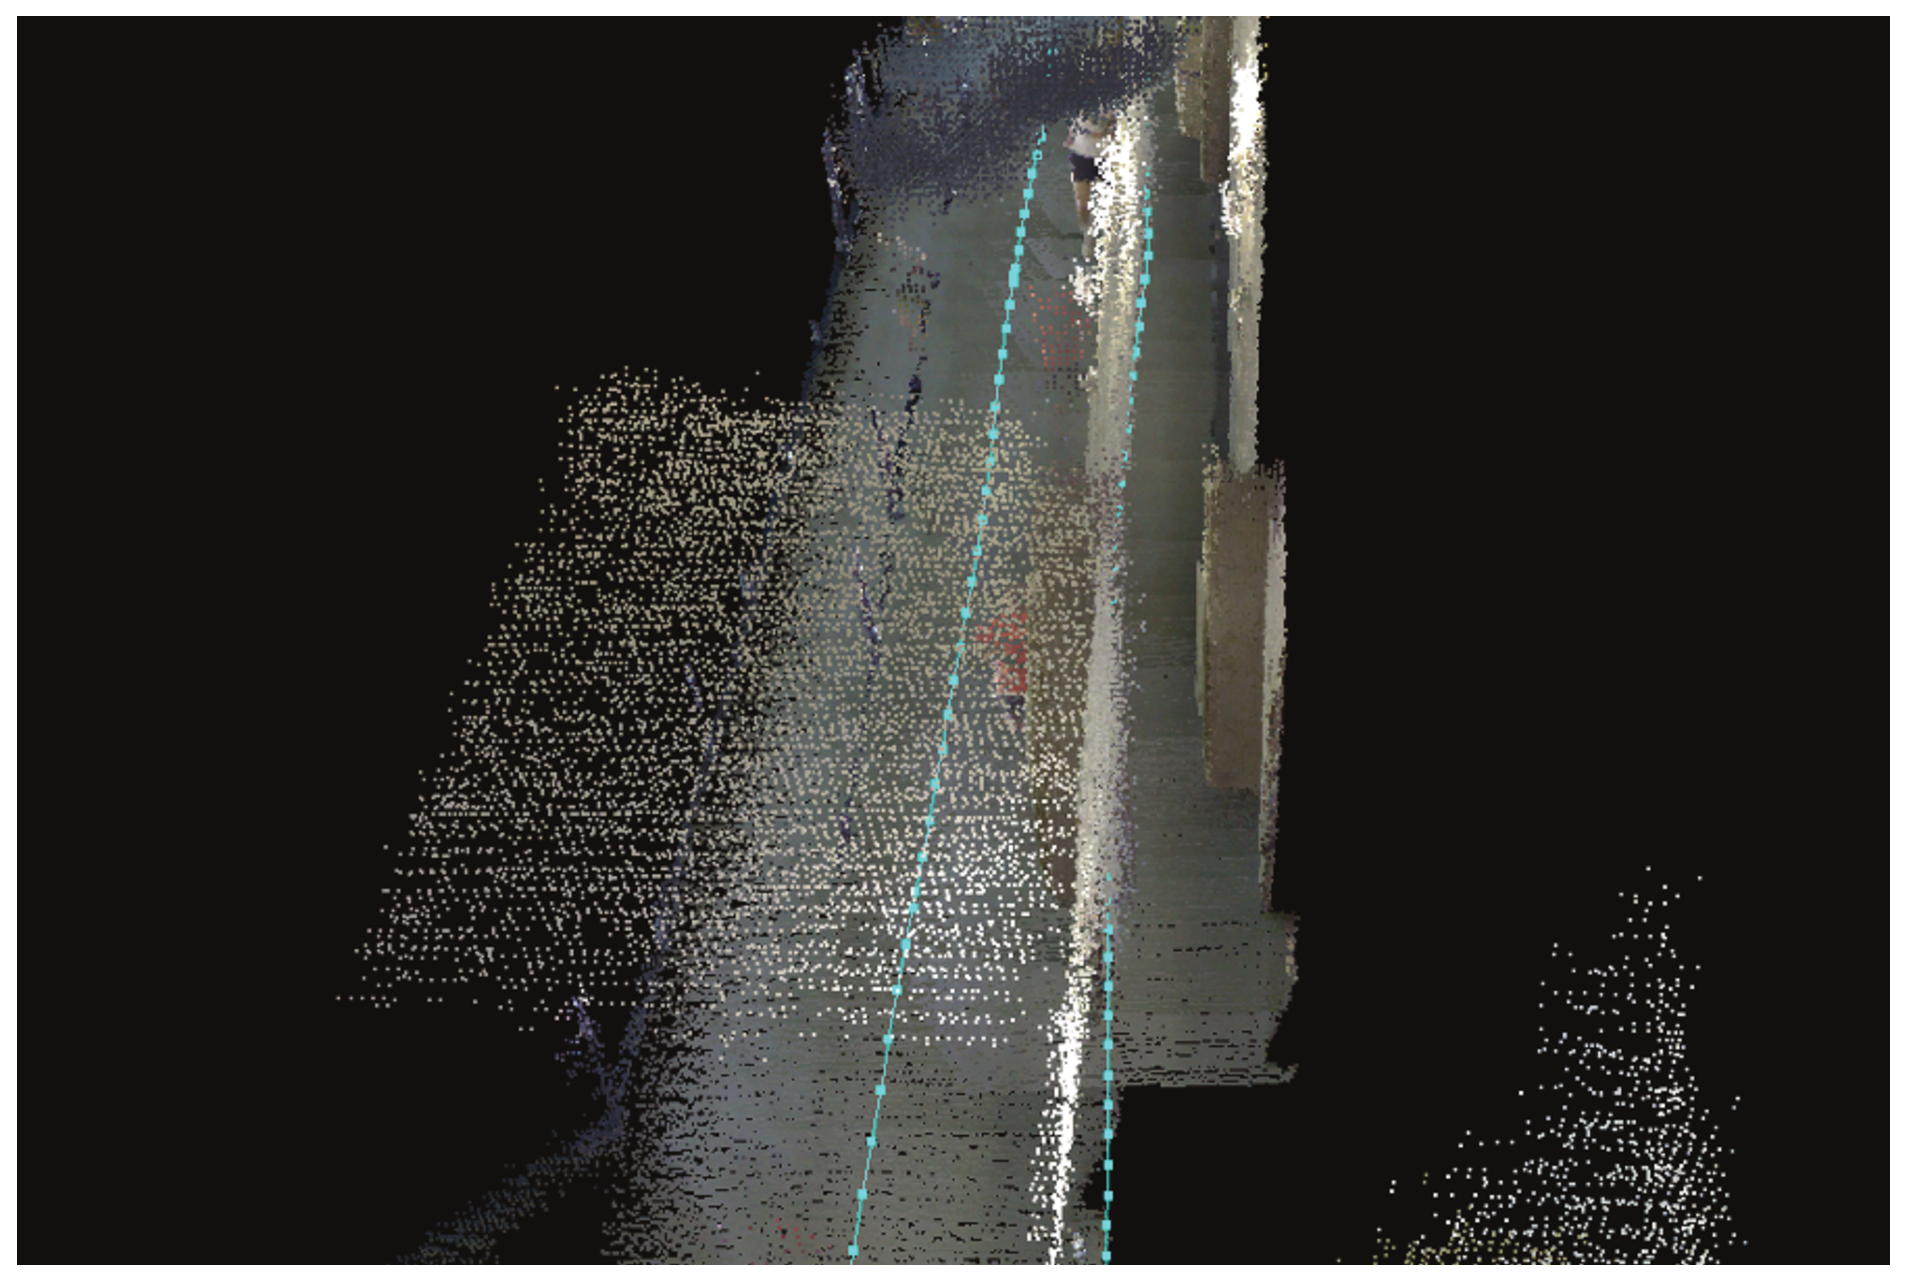
\includegraphics[height=1.0in]{Figure9_e.eps}
   % \hspace{.2in}
    %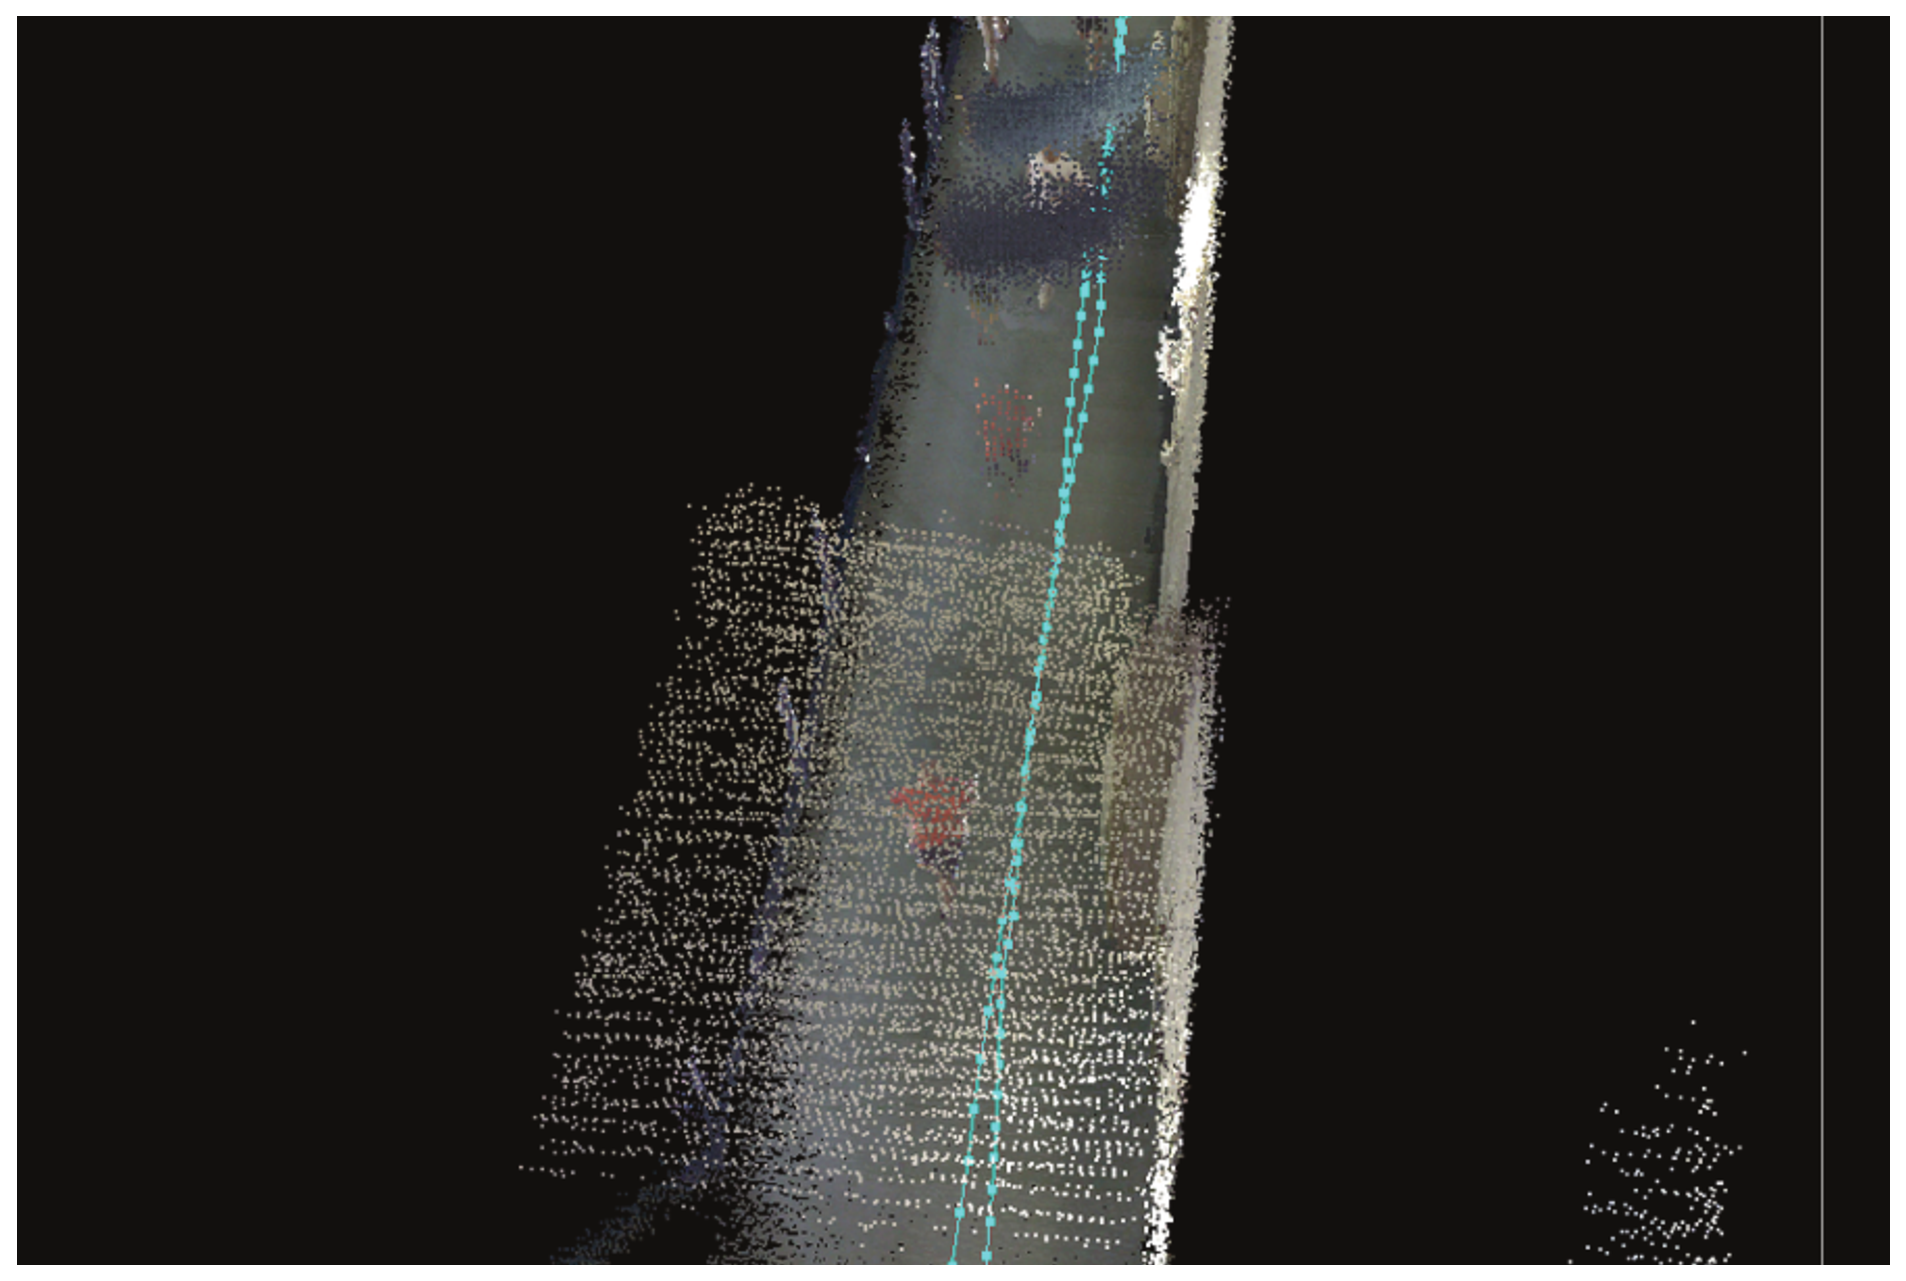
\includegraphics[height=1.0in]{Figure9_f.eps}
%\caption{Constructed maps of J Hall (top row) and A Hall (center row) using original RTAB-Map (left) and Wi-Fi augmented RTAB-Map (right).  The cropped images (bottom row) are the portion of the map from A Hall (center row) highlighted in the red rectangle. They show the difference in constructed map without loop closure in original approach (left) and with correct loop closures in Wi-Fi RTAB-Map (right)}
\caption{Constructed maps of J Hall (top row) using original RTAB-Map (left) and Wi-Fi augmented RTAB-Map (right). They show the difference in constructed map without loop closure in original approach (left) and with correct loop closures in Wi-Fi RTAB-Map (right)}
\label{fig:rtabmap_maps_2}
%\vspace{-10pt}
\end{figure}
\begin{table*}
\caption{{\bf RTAB-Map:} Trajectory error (m) for different datasets and different {\it real-time thresholds}}
\begin{center}
\begin{tabular}{| c | r r | r r | r r | r r | } 
\hline 
\multicolumn{9}{|c|}{Real-time Threshold (ms)} \\ 
\hline 
 & \multicolumn{2}{|c|}{$\infty$} & \multicolumn{2}{|c|}{70} & \multicolumn{2}{|c|}{100} & \multicolumn{2}{|c|}{200} \\ 
\hline 
 Dataset & \multicolumn{1}{|c|}{Vanilla} & \multicolumn{1}{|c|}{WiFi} & \multicolumn{1}{|c|}{Vanilla} & \multicolumn{1}{|c|}{WiFi} & \multicolumn{1}{|c|}{Vanilla} & \multicolumn{1}{|c|}{WiFi} & \multicolumn{1}{|c|}{Vanilla} & \multicolumn{1}{|c|}{WiFi} \\ 
\hline 
 A Hall & 0.23 & 0.22 & 0.48 & 0.25 & 0.48 & 0.28 & 0.23 & 0.20 \\ 
 B Hall & 0.24 & 0.22 & 0.12 & 0.22 & 0.12 & 0.22 & 0.19 & 0.22 \\ 
 C Hall & 0.12 & 0.11 & 0.11 & 0.10 & 0.11 & 0.10 & 0.11 & 0.14 \\ 
 J Hall & 0.30 & 0.21 & 1.34 & 0.19 & 1.34 & 0.19 & 0.23 & 0.21 \\ 
\hline 
\end{tabular} 
\label{table:rtabmap_rmse}
\end{center}
%\vspace{-10pt}
\end{table*}

\begin{table*}
\caption{{\bf RTAB-Map:} False negative loop closures for different datasets and different {\it real-time thresholds}}
\begin{center}
\begin{tabular}{| c | r r | r r | r r | r r | } 
\hline 
\multicolumn{9}{|c|}{Real-time Threshold (ms)} \\ 
\hline 
 & \multicolumn{2}{|c|}{$\infty$} & \multicolumn{2}{|c|}{70} & \multicolumn{2}{|c|}{100} & \multicolumn{2}{|c|}{200} \\ 
\hline 
 Dataset & \multicolumn{1}{|c|}{Vanilla} & \multicolumn{1}{|c|}{WiFi} & \multicolumn{1}{|c|}{Vanilla} & \multicolumn{1}{|c|}{WiFi} & \multicolumn{1}{|c|}{Vanilla} & \multicolumn{1}{|c|}{WiFi} & \multicolumn{1}{|c|}{Vanilla} & \multicolumn{1}{|c|}{WiFi} \\ 
\hline 
 A Hall & 0.00 & 4.44 & 100.00 & 17.77 & 100.00 & 31.11 & 11.11 & 13.33 \\ 
 B Hall & 8.00 & 16.00 & 100.00 & 0.00 & 100.00 & 0.00 & 6.00 & 12.00 \\ 
 C Hall & 6.06 & 0.00 & 100.00 & 9.09 & 100.00 & 9.09 & 27.27 & 3.03 \\ 
 J Hall & 9.09 & 9.09 & 100.00 & 13.63 & 100.00 & 40.90 & 0.00 & 9.09 \\ 
\hline 
\end{tabular} 
\label{table:rtabmap_false_negative}
\end{center}
%\vspace{-20pt}
\end{table*}
RTAB-Map is another state-of-the-art SLAM system. A key parameter in RTAB-Map is the ability to control the running time of the algorithm by setting {real-time threshold} parameter. 
The algorithm tries to keep the processing time of each node under {real-time threshold} by moving unused frames to LTM only to retrieving them back when necessary. 
In our experiments, we set different real-time threshold values and compare the behavior of vanilla RTAB-Map with our proposed approach for different datasets. 
We note that {real-time threshold}=$\infty$ means no threshold is set and no frame is moved to LTM.

Table~\ref{table:rtabmap_rmse} represents the trajectory error of both original and Wi-Fi augmented RTAB-Map for different datasets and {real-time thresholds}. 
For {real-time thresholds} of $\infty$ and 200, the trajectory error of both approaches is on the same order.
This is because of the number of frames moved to LTM. For a value of 0, no frame is moved to LTM. 
For a value of 200, the number of transferred frames is too low, because the processing time of most of the frames is less than this threshold.
Some of the error differences for these two real-time threshold values are due to the randomness of matched frames. 
Among a set of consecutive frames, selecting either one for loop closure may result in a slightly different visual transformation. 
For {real-time thresholds} of 70 and 100, the original approach is not able to detect any loop closure, because all the related nodes are transferred to LTM. 
But in our approach, we are able to retrieve back the transferred nodes to WM using Wi-Fi sensing. 
So we are able to make correct loop closures and experience a much smaller trajectory error, especially in A Hall and J Hall. 
These two datasets are very large and odometry measurements are subject to noise accumulation. 
Therefore, a correct loop closure benefits the localization accuracy to a high extent. 
Figure~\ref{fig:rtabmap_maps_2} presents the constructed maps of both approaches for J Hall in {real-time threshold}=70. % and A Hall 
For B Hall, the results show a lower error for vanilla RTAB-Map. 
We believe this stems from the small size of the dataset. 
Because in vanilla RTAB-Map, the trajectory error of B hall with no loop closure in {real-time threshold} of 70 and 100 is less than the case with correct detected loop closures with {real-time threshold}=$\infty$ when no frame is transferred to LTM. 
%This case approves our belief about the role of odometry in small environments.
In such an environment, the odometry may be able to provide a more accurate trajectory than visual estimations. 

Table~\ref{table:rtabmap_false_negative} shows the percentage of false negative loop closures of each approach for different {real-time threshold} values. 
For {real-time threshold}=200 and {real-time threshold}=$\infty$, the percentage of false negatives of both approaches is less than 20.
This is due to infrequent or no frame transfers to LTM.
Percentage values higher than zero in {real-time threshold}=$\infty$, where no frames are transferred to LTM, show that several loop closures are missed due to the random absence of some visual features in multiple frames.
As shown, all the possible correct loop closures are missing in the original approach for {real-time thresholds} of 70 and 100 due to unavailability of corresponding frames in WM. 
Two conditions lead to non-zero percentage values in our approach: 1- Random absence of visual features in some frames, 2- Availability of frames in WM; different pools of frames in WM generate different loop closure candidates.
% \zaki{Two conditions lead to non-zero percentage values in our approach: 1- Random absence of visual features, 2- Applying normalization and Bayes estimation for finding the best candidate for loop closure which is dependent on which frames are available in WM, and different subsets could lead to different calculations and candidate selection. %Time and position of pause points which could cause a small delay in frame retrieval from LTM.
%For avoiding the second condition, more frequent pause points could be solution and a trade off between operation runtime and accuracy should be adjusted.
But based on results in Table~\ref{table:rtabmap_rmse}, low percentage of false negatives doesn't affect the trajectory accuracy.
We don't see any specific reason for higher percentage values of A and J Hall datasets for {real-time threshold} of 100 except the above conditions.
Since there are no false positive loop closures detected in either approach in RTAB-Map, no results are shown.   
\begin{table*}
\caption{{\bf RTAB-Map:} Loop closure compute time (s) for different datasets with different {\it real-time thresholds} }
\begin{center}
\begin{tabular}{| c | r r | r r | r r | r r | } 
\hline 
\multicolumn{9}{|c|}{Real-time Threshold (ms)} \\ 
\hline 
 & \multicolumn{2}{|c|}{$\infty$} & \multicolumn{2}{|c|}{70} & \multicolumn{2}{|c|}{100} & \multicolumn{2}{|c|}{200} \\ 
\hline 
 Dataset & \multicolumn{1}{|c|}{Vanilla} & \multicolumn{1}{|c|}{WiFi} & \multicolumn{1}{|c|}{Vanilla} & \multicolumn{1}{|c|}{WiFi} & \multicolumn{1}{|c|}{Vanilla} & \multicolumn{1}{|c|}{WiFi} & \multicolumn{1}{|c|}{Vanilla} & \multicolumn{1}{|c|}{WiFi} \\ 
\hline 
 A Hall & 7.11 & 2.35 & 3.57 & 5.05 & 3.74 & 5.02 & 6.95 & 3.99 \\ 
 B Hall & 2.36 & 0.63 & 4.67 & 1.85 & 4.93 & 1.88 & 2.61 & 1.69 \\ 
 C Hall & 1.69 & 0.62 & 4.90 & 1.66 & 4.71 & 1.67 & 3.50 & 1.38 \\ 
 J Hall & 4.72 & 0.80 & 7.57 & 2.60 & 6.75 & 2.64 & 4.49 & 2.81 \\ 
\hline 
\end{tabular} 
\label{table:rtabmap_bounding}
\end{center}
%\vspace{-15pt}
\end{table*} 

In Table~\ref{table:rtabmap_bounding}, we show the computation time of loop closure detection for both approaches and all datasets. 
{Bounding loop closure} is supposed to save computation time in this process by restricting the number of comparisons. 
The results confirm that almost for all datasets and {\it real-time thresholds}, we are spending much less time for loop closure detection. 
The only different cases are for very long A dataset for {\it real-time thresholds} of 70 and 100. 
This is due to the size and shape of the environment. 
The A Hall dataset is very large and there are not many blocking walls along the trajectory which causes less RSSI attenuation between different places. 
This leads to less number of Wi-Fi clusters. 
As previously mentioned, there are only 8 Wi-Fi clusters created in this very large environment while the same number for smaller J and B datasets are 19 and 13. 
A low number of Wi-Fi clusters in a large environment lead to a very high number of keyframes in each cluster. 
In this situation, visual comparison to even one single {similar cluster} takes more time while the original approach is transferring many nodes to LTM due to the low {\it real-time threshold} and does a very low number of visual comparisons.

\zaki{It should be noted that if we increase the Wi-Fi similarity threshold, the number of clusters would increase which may help in reducing the loop closure computation time. But it would also decrease the number of detected similar clusters for each frame which may lead to loosing some correct loop closures.}

\begin{table}
\caption{{\bf RTAB-Map:} Compute overheadi (s) of {Wi-Fi clustering} and {cluster management} for different datasets and different {\it real-time thresholds}}
\begin{center}
\begin{tabular}{| c | r | r | r | r | } 
\hline 
\multicolumn{5}{|c|}{Real-time Threshold (ms)} \\ 
\hline 
 & \multicolumn{1}{|c|}{$\infty$} & \multicolumn{1}{|c|}{70} & \multicolumn{1}{|c|}{100} & \multicolumn{1}{|c|}{200} \\ 
\hline 
 {Dataset} & \multicolumn{1}{|c|}{WiFi} & \multicolumn{1}{|c|}{WiFi} & \multicolumn{1}{|c|}{WiFi} & \multicolumn{1}{|c|}{WiFi} \\ 
\hline 
 A Hall & 0.32 & 0.34 & 0.34 & 0.33 \\ 
 B Hall & 0.21 & 0.22 & 0.22 & 0.21 \\ 
 C Hall & 0.17 & 0.17 & 0.18 & 0.16 \\ 
 J Hall & 0.56 & 0.63 & 0.62 & 0.62 \\ 
\hline 
\end{tabular} 
\label{table:rtabmap_overhead}
\end{center}
%\vspace{-10pt}
\end{table}
Table~\ref{table:rtabmap_overhead} represents the computation overhead of our approach for all datasets caused by {\it Wi-Fi Clustering} and {\it Cluster Management} modules. 
As shown, these overheads are very small and could be ignored with respect to saved computation time shown in Table~\ref{table:rtabmap_bounding}. 
Based on the shown result, the amount of computation overhead is dependent on both the number of Wi-Fi clusters and the size of the dataset (number of frames). 
Higher number of clusters and higher number of frames lead to more comparisons and more computation overhead as expected. 
So although B dataset has a higher number of clusters than A dataset, it has a lower computation overhead due to less number of frames (748 compared to 1270).

\begin{table*}
\caption{{\bf ORB-SLAM:} Trajectory error (m) of different datasets and different {\it min-matches} values}
\begin{center}
\begin{tabular}{| c | r r | r r | r r | r r | r r |} 
\hline 
\multicolumn{11}{|c|}{{Min-Matches}} \\ 
\hline 
 & \multicolumn{2}{|c|}{10} & \multicolumn{2}{|c|}{15} & \multicolumn{2}{|c|}{20} & \multicolumn{2}{|c|}{50} & \multicolumn{2}{|c|}{100} \\ 
\hline 
 {Dataset} & \multicolumn{1}{|c|}{Vanilla} & \multicolumn{1}{|c|}{WiFi} & \multicolumn{1}{|c|}{Vanilla} & \multicolumn{1}{|c|}{WiFi} & \multicolumn{1}{|c|}{Vanilla} & \multicolumn{1}{|c|}{WiFi} & \multicolumn{1}{|c|}{Vanilla} & \multicolumn{1}{|c|}{WiFi} & \multicolumn{1}{|c|}{Vanilla} & \multicolumn{1}{|c|}{WiFi} \\ 
\hline 
 B Hall & 10.96 & 0.21 & 10.09 & 0.23 & 0.25 & 0.23 & 0.21 & 0.20 & 0.41 & 0.45 \\ 
 C Hall & 12.22 & 0.16 & 13.50 & 0.15 & 0.11 & 0.09 & 0.21 & 0.20 & 0.33 & 0.38 \\ 
 J Hall & 0.86 & 0.86 & 0.82 & 0.73 & 0.74 & 0.66 & 0.85 & 0.77 & 2.72 & 2.84 \\ 
 \hline 
 \end{tabular}
\label{table:orbslam_rmse}
\end{center}
%\vspace{-20pt}
\end{table*}
\subsection{ORB-SLAM performance}
%ORB-SLAM is one of the most recent SLAM algorithms. In this approach, they use a visual word dictionary in order to find loop closure candidates for the current frame. Although ORB-SLAM seems very accurate in map construction, but it yet could suffer from perceptual aliases. In order to show the applicability of our proposed method for ORB-SLAM, we try different {min-matches} values. This parameter specifies the minimum number of required inliers in RANSAC algorithm for accepting a visual transformation.

For ORB-SLAM, the tunable parameter is {\it min-matches} which is the number of inliers required in matching frames to accept a visual transformation. 
{\bf NOTE}: We were not able to get any result for A Hall in ORB-SLAM due to it having very low number of features.

Table~\ref{table:orbslam_rmse} shows the error of estimated trajectories for different {\it min-matches}. 
B Hall and C Hall experience false positive loop closures for {\it min-matches} of 10 and 15. 
So the estimated trajectories are inaccurate.
But we are able to avoid any false positive loop closure even with low values for {\it min-matches}. 
This shows that our proposed approach is applicable in symmetric environments having similar looking scenes. 
For higher values of {\it min-matches}, the trajectory error of both approaches is similar to each other.
In {\it min-matches}=100, the trajectory error is higher than in other settings. This is due to having a lower number of permissible visual transformations and more false negatives.
\begin{table*}
\caption{{\bf ORB-SLAM:} Loop closure compute time (s) for different datasets and different {\it min-matches} values. Our method reduces this time by 15\%-25\% on average. }
\begin{center}
\begin{tabular}{| c | r r | r r | r r | r r | r r |} 
\hline 
\multicolumn{11}{|c|}{{Min-Matches}} \\ 
\hline 
 & \multicolumn{2}{|c|}{10} & \multicolumn{2}{|c|}{15} & \multicolumn{2}{|c|}{20} & \multicolumn{2}{|c|}{50} & \multicolumn{2}{|c|}{100} \\ 
\hline 
 {Dataset} & \multicolumn{1}{|c|}{Vanilla} & \multicolumn{1}{|c|}{WiFi} & \multicolumn{1}{|c|}{Vanilla} & \multicolumn{1}{|c|}{WiFi} & \multicolumn{1}{|c|}{Vanilla} & \multicolumn{1}{|c|}{WiFi} & \multicolumn{1}{|c|}{Vanilla} & \multicolumn{1}{|c|}{WiFi} & \multicolumn{1}{|c|}{Vanilla} & \multicolumn{1}{|c|}{WiFi} \\ 
\hline 
 B Hall & 10.09 & 7.04 & 9.68 & 7.29 & 9.10 & 6.50 & 8.91 & 7.11 & 9.23 & 7.69 \\ 
 C Hall & 19.03 & 16.49 & 19.67 & 15.90 & 21.17 & 18.84 & 18.27 & 15.78 & 18.50 & 15.58 \\ 
 J Hall & 25.28 & 19.63 & 25.37 & 20.08 & 24.96 & 19.99 & 25.32 & 20.32 & 24.68 & 19.79 \\ 
\hline 
\end{tabular}  
\label{table:orbslam_bounding}
\end{center}
%\vspace{-20pt}
\end{table*}

In Table~\ref{table:orbslam_bounding}, we show the processing time of loop closure detection in the original approach and in our approach. 
Results show that for a similar level of accuracy in Table~\ref{table:orbslam_rmse}, we spend less time (15\%-25\% on average) for loop closure detection resulting in faster execution.
The difference in computation time grows larger as the dataset gets bigger(J Hall compared to B and C Hall). 
The reason is that the original approach always searches through all keyframes, but our approach is able to bound the searching process to keyframes of regions spatially close to current frame using Wi-Fi sensing. 
Further, the false positive loop closures increase the computation time by running global bundle adjustment wrongly. 
This shows that our Wi-Fi sensing is able to save time in the optimization process by avoiding false loop closures as well.  
\begin{table}[t]
\caption{{\bf ORB-SLAM:}Compute overhead (s) of {\it Wi-Fi Clustering} and {\it Cluster Management} modules for different datasets and {\it min-matches} values. It is about 3\%-8\% on average. }
\begin{center}
\begin{tabular}{| c | r | r | r | r | r |} 
\hline 
\multicolumn{6}{|c|}{{Min-Matches}} \\ 
\hline 
 & \multicolumn{1}{|c|}{10} & \multicolumn{1}{|c|}{15} & \multicolumn{1}{|c|}{20} & \multicolumn{1}{|c|}{50} & \multicolumn{1}{|c|}{100} \\ 
\hline 
{Dataset} & \multicolumn{1}{|c|}{WiFi} & \multicolumn{1}{|c|}{WiFi} & \multicolumn{1}{|c|}{WiFi} & \multicolumn{1}{|c|}{WiFi} & \multicolumn{1}{|c|}{WiFi} \\ 
\hline 
 B Hall & 0.42 & 0.46 & 0.41 & 0.45 & 0.53 \\ 
 C Hall & 0.49 & 0.39 & 0.44 & 0.65 & 0.46 \\ 
 J Hall & 1.75 & 1.65 & 1.59 & 1.70 & 1.77 \\ 
\hline 
\end{tabular} 
\label{table:orbslam_overhead}
\end{center}
%\vspace{-10pt}
\end{table}

Table~\ref{table:orbslam_overhead} represents the computation time overhead caused by {\it Wi-Fi Clustering} and {\it Cluster Management} modules in our approach. 
As shown in Table~\ref{table:orbslam_bounding}, the computation time savings far outweigh these overhead values. 
These overhead values are dependent on the number of keyframes and Wi-Fi clusters. 
J dataset has a little more overhead due to more number of keyframes(about 2800) and 19 Wi-Fi clusters. 
B and C datasets are analogous to each other due to some randomness in their number of keyframes for different values of {\it min-matches}. 
For example for {\it min-matches}=50, the respective keyframes of B and C datasets are 1200 and 1500. 
So although C dataset has a lower number of Wi-Fi clusters, it has more computation overhead. 
\begin{table}[t]
\caption{{\bf ORB-SLAM:} Percentage false positive loop closures for different datasets and different {\it min-matches} values. Our method has zero false positives and is therefore not shown in the table. }
\begin{center}
\begin{tabular}{| c | r | r | r | r | r |} 
\hline 
\multicolumn{6}{|c|}{{Min-Matches}} \\ 
\hline 
 & \multicolumn{1}{|c|}{10} & \multicolumn{1}{|c|}{15} & \multicolumn{1}{|c|}{20} & \multicolumn{1}{|c|}{50} & \multicolumn{1}{|c|}{100} \\ 
\hline 
 {Dataset} & \multicolumn{1}{|c|}{Vanilla} & \multicolumn{1}{|c|}{Vanilla} & \multicolumn{1}{|c|}{Vanilla} & \multicolumn{1}{|c|}{Vanilla} & \multicolumn{1}{|c|}{Vanilla} \\ 
\hline 
 B Hall & 40.00 & 33.30 & 0.00 & 0.00 & 0.00 \\ 
 C Hall & 50.00 & 50.00 & 0.00 & 0.00 & 0.00 \\ 
 J Hall & 0.00 & 0.00 & 0.00 & 0.00 & 0.00 \\  
\hline 
\end{tabular} 
\label{table:orbslam_false_positive}
\end{center}
%\vspace{-10pt}
\end{table}

In Table~\ref{table:orbslam_false_positive}, we show the percentage of false positive loop closures with respect to all detected ones in each parameter setting. 
As discussed earlier, B and C dataset suffer from some false positives for {\it min-matches} $\in (10, 15)$. %values of 10 and 15. 
This shows the vulnerability of the original approach to symmetric environments and demonstrates the ability of our version of ORB-SLAM to work well even when the {\it min-matches} value is low. 
Our approach using Wi-Fi does not incur any false positives for loop closure detection and is therefore not shown in the table. 
Also, there are no false negatives observed in any settings except for {\it min-match}=100 which is equal for both approaches.
%This could help compute time as it reduces the overhead of loop closure matching as shown in Table~\ref{table:orbslam_bounding} 
%i.e., for a similar level of accuracy, our algorithm could use a lower value for {\it min-matches} resulting in faster execution. 
%\vspace{-5pt}
\subsection{Comparison to Wi-Fi augmented FABMAP}
\begin{figure*}
	\begin{subfigure}[b]{.24\textwidth}
		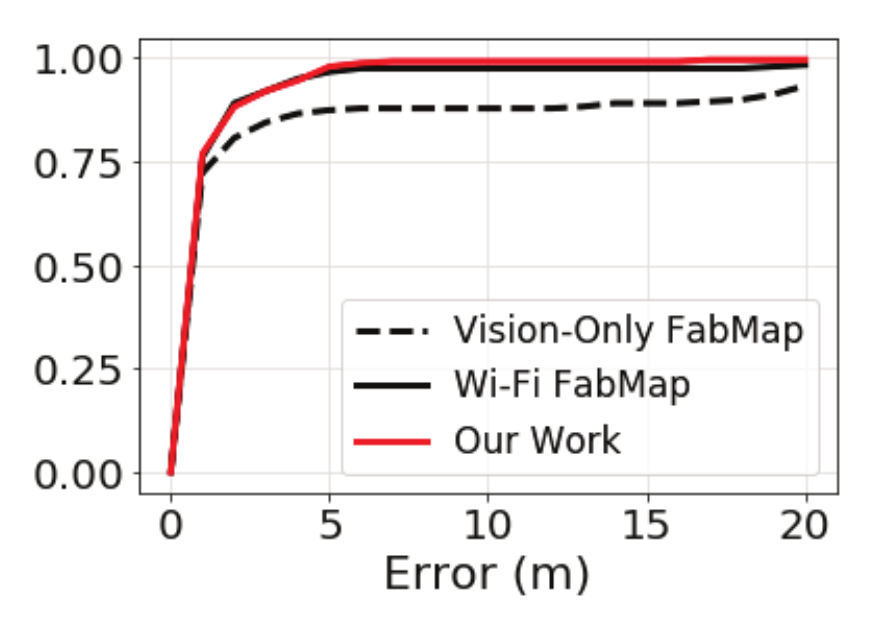
\includegraphics[width=\textwidth]{Figure10_a.eps}
		%\label{subfig:center}
		%\vspace{-6mm}
		\caption{C Hall}
	\end{subfigure}
	\begin{subfigure}[b]{0.24\textwidth}
		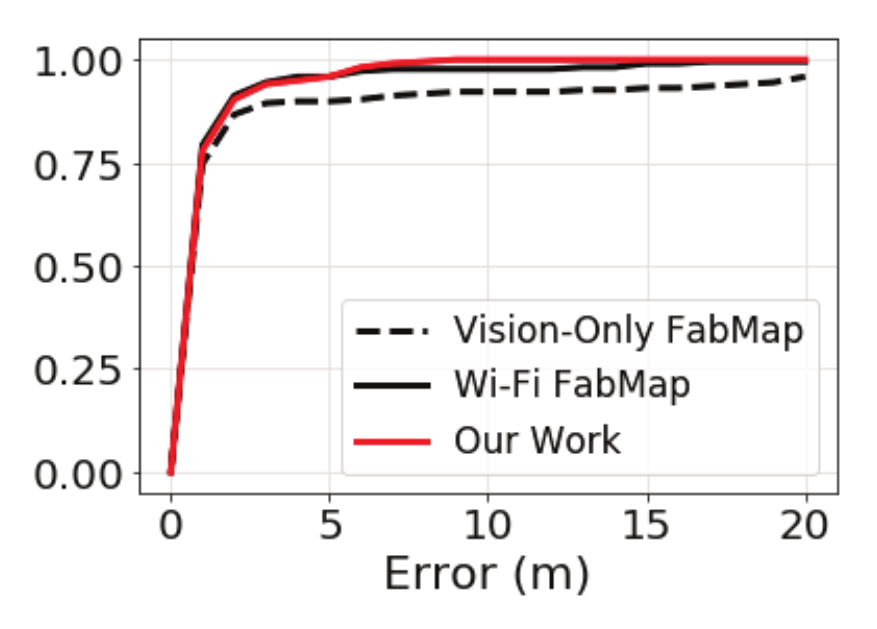
\includegraphics[width=\textwidth]{Figure10_b.eps}
		%\label{subfig:center}
		%\vspace{-6mm}
		\caption{B Hall}
	\end{subfigure}
	\begin{subfigure}[b]{0.24\textwidth}
		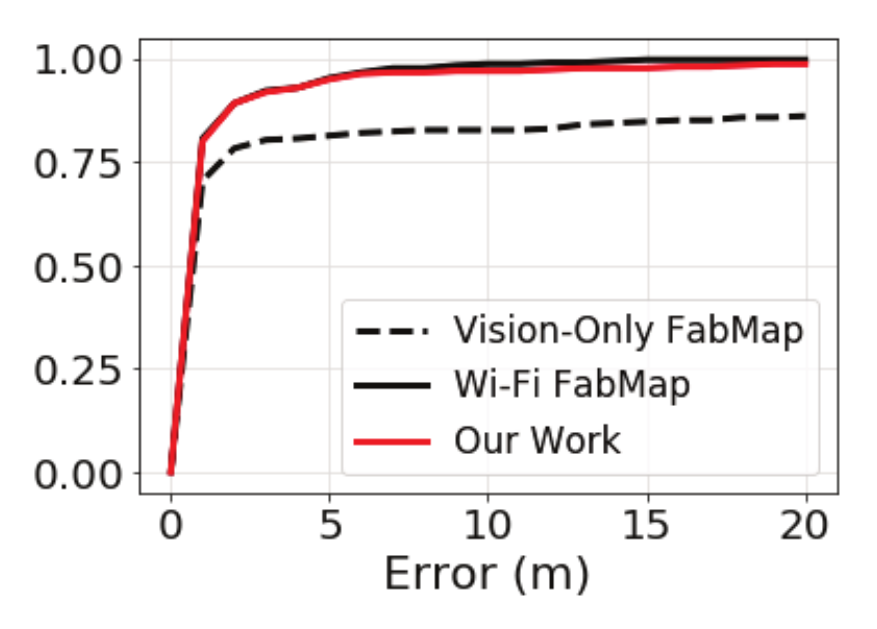
\includegraphics[width=\textwidth]{Figure10_c.eps}
		%\label{subfig:center}
		%\vspace{-6mm}
		\caption{J Hall}
	\end{subfigure}
	\begin{subfigure}[b]{0.24\textwidth}
		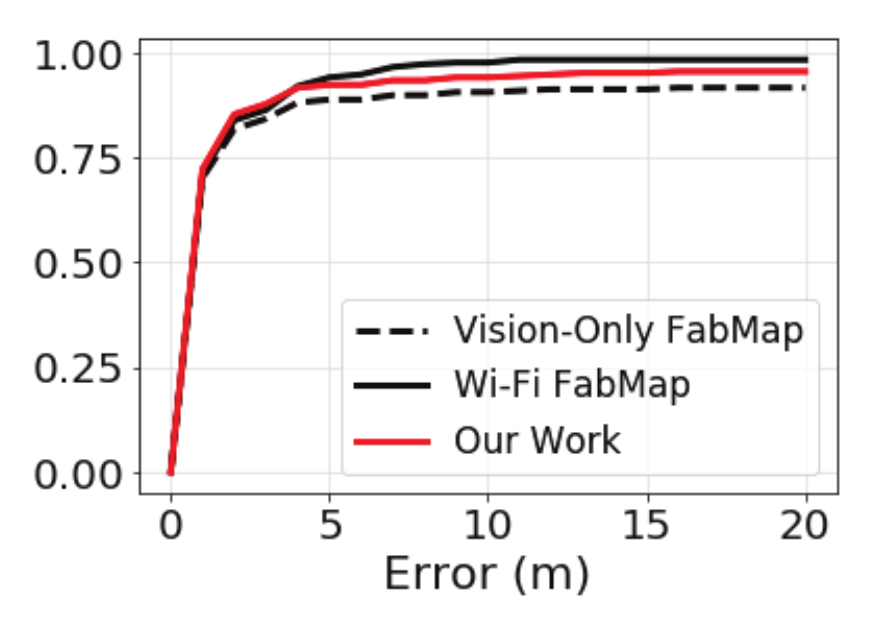
\includegraphics[width=\textwidth]{Figure10_d.eps}
		%\label{subfig:center}
		%\vspace{-6mm}
		\caption{A Hall}
	\end{subfigure}
%\vspace{-10pt}
\caption{CDF of Error in Wi-Fi augmented FABMAP compared to our approach}
\label{fabmap}
%\vspace{-10pt}
\end{figure*}
To situate our work wrt other visual SLAM algorithms that integrate Wi-Fi, we chose Wi-Fi FABMAP~\cite{visual_wifi_2}, the most recent work
that we came across that integrates wireless sensing with a specific visual SLAM algorithm. 

Wi-Fi augmented FABMAP~\cite{visual_wifi_2} is a topological localization algorithm which introduces a new approach for early fusion of visual and Wi-Fi information. It is executed in two phases: the mapping phase and the localization phase.
In the mapping phase, the robot is driven through the target area to collect Wi-Fi AP MAC addresses and images of the environment.
In this phase, each image is assumed to be from a different location and is associated with the spatially closest collected Wi-Fi vector, which is a binary vector indicating the presence of APs.
In the localization phase, the feature vector extracted from the query image is concatenated with the Wi-Fi vector collected at the location and fed into the FABMAP algorithm to find the best match among the images collected during the mapping phase.

{\bf Note:} (i) it is a two-phased method that requires war-driving. (ii) Wi-Fi FABMAP does not use signal strength values. Instead, it simply creates the Wi-Fi vector as a vector of binary values indicating the presence or absence of APs. (iii) It uses the Wi-Fi information only in the localization phase as opposed to integrating it into the SLAM process.

%\footnote{We spent some time on an available GitHub repo (\url{https://github.com/LRMPUT/WiFi-FAB-MAP}) but could not get it to work properly}
We faithfully re-implemented their algorithm by adapting the available open source code-base for FABMAP~\cite{glover2012openfabmap}. We collected data for input as per their paper by acquiring images every 2s and Wi-Fi data every 10s while the robot is in motion. The collected data is split into two sets: around 40\% for the mapping phase and 60\% for the localization phase. We also associated the Wi-Fi data with the images as per the procedure mentioned separately for the two phases.
The visual vocabulary was learned from 1500 images of corridor scenes from~\cite{yang_icra16,quattoni_cvpr09} and self-collected images in our university.

%Since topological SLAM, like FabMap, is different from metric SLAM,
FABMAP is a topological SLAM algorithm and not a metric SLAM algorithm such as RTAB-Map, and ORB-SLAM. Therefore, FABMAP and its derivatives would perform poorly in direct localization or mapping error comparison. For a fairer comparison, {\it we chose the exact same metrics} as used in~\cite{visual_wifi_2}. 
 %We chose to use the metric used in~\cite{visual_wifi_2} rather than the metrics used for RTABMap and ORB-SLAM comparisons. 
This is the \zaki{Cumulative Distance Function}(CDF) of distances between the estimated location and ground-truth averaged over the query images. To enable this comparison, we also provide localization results from our method over the query images rather than produce a trajectory.
In our approach, we use Wi-Fi signatures, which is a vector of RSSI values, rather than a binary vector used by Wi-Fi augmented FABMAP. We first find a representative Wi-Fi signature for each Wi-Fi cluster and the time stamp associated with it. %We assign this signature to all map images based on their time stamps. 
Then we associated every map image to a specific cluster based on their acquisition time stamps. For localization, the query image is also assigned a Wi-Fi signature. This is the signature recorded at the last pause prior to its acquisition. 
To get the best map image matching the query image, we first select clusters that their representative Wi-Fi signatures have high cosine similarity with the Wi-Fi signature of the query image named {\it similar clusters}. Then among the map images associated with similar clusters, we select the map image with maximum visual likelihood with the query image.%an image from the clusters based on the visual likelihood comparison with the query image.

%As mentioned previously, we use the metrics and illustrations similar to~\cite{visual_wifi_2} in this section. 
Figure~\ref{fabmap} shows the CDF of error between estimated localization and ground-truth of our Wi-Fi clustering method, Wi-Fi augmented FABMAP and visual FABMAP for all four datasets. We perform better for Halls B and C because:
\begin{itemize}
\item In some instances, the high similarity in visual features from physically different locations causes the algorithm to make the wrong matches even with the Wi-Fi data.
\item The constructed Wi-Fi Chow Liu tree could be inaccurate in capturing relations due to using raw Wi-Fi data.
The randomness associated in the detection of APs over time could cause the Chow Liu tree to have dependencies that don't necessarily hold.
Using our approach and aggregating the BSSIDs differing only in the last nibble could reduce the problem.
\end{itemize}
Our performance is similar to~\cite{visual_wifi_2} for J Hall. For Hall A, Wi-Fi augmented FABMAP performs better. The reason for this is that A Hall is a wide area with fewer features that doesn't include many blocking objects like walls along the trajectory. This causes less RSSI attenuation and therefore lesser number of Wi-Fi cluster. Since there are fewer clusters, there are more images per cluster and this increases the chances for perceptual aliasing. But we do note that even under these circumstances, more than 90\% of the query images are within 4 meters accuracy which is similar to Wi-Fi augmented FABMAP.

In summary, the demonstrated results show our performance improvement, in terms of localization/mapping accuracy and computational complexity, in visual SLAM algorithms.
% This improvement is due the employment of the unique features of Wi-Fi data in a well-suited and generic way in the original approaches.
The low dimensionality of Wi-Fi data and its immunity to perceptual aliasing are the key elements of the performance gain.
Further, the comparison with the state-of-the-art Wi-Fi FABMAP, shows a similar if not better performance.
This shows the generality of our approach unlike Wi-Fi augmented FABMAP which is specifically designed for visual FABMAP.
% \zaki{
% Wi-Fi augmented FabMap~\cite{visual_wifi_2} is a recent topological localization algorithm which introduces a new approach for early fusion of visual and Wi-Fi information.
% In their method, first they employ an initial mapping phase for generating a map of Wi-Fi and visual information of the respective environment.
% In this phase, each image is considered as a new place and is associated to the spatially closest collected Wi-Fi signature.
% In the second phase for global localization, they associate each query image to the last Wi-Fi signature acquired, concatenate the respective observed visual and Wi-Fi vectors, and feed the constructed observation vector to FabMap algorithm for finding the best match in the map images. 
% So Wi-Fi information is only utilized in global localization phase.
% They also ignore the RSSI values and only use binary values to indicate the presence or absence of BSSID addresses.
%
% In order to compare our approach to Wi-Fi FabMap, we faithfully implemented their algorithm by adapting the available open source code-base~\cite{glover2012openfabmap}.
% For providing input data, we followed their procedure and acquired images every 2s and Wi-Fi data every 10s while our robot was moving and didn't use any data while it was pausing.
% Then the acquisitions were split in two: around 40\% were used for mapping and 60\% for global localization.
% The association between image and Wi-Fi data also follows their routines separately for mapping and localization phase.
%
% For comparison between the two approaches in terms of localization accuracy, we couldn't directly use our result from Wi-Fi augmented RTABMap or ORB-SLAM.
% Because not only the data collection routine differs between the two approaches, but also comparison among metric SLAM and topological localization is not very acceptable.
% In order to enable a fair comparison, we had to apply our Wi-Fi clustering method on the images used for mapping in Wi-Fi FabMap.
% Then in the localization phase, we would compare each query image only to images within similar Wi-Fi clusters.
%
% For this purpose, we recorded the representative Wi-Fi signatures of all constructed Wi-Fi clusters and their corresponding time stamps in our approach.
% Using the recorded time stamps of our Wi-Fi clusters and the time stamps of map images in Wi-Fi FabMap, we were able to assign each map image to its corresponding Wi-Fi cluster.
% Each map image was associated to the last constructed Wi-Fi cluster before acquiring the respective image.
%
% In the next step for global localization, we recorded the Wi-Fi signatures computed after each pause point and their corresponding time stamps in our approach. 
% We associated each query image to the computed Wi-Fi signature of the last pause point before its respective acquisition time stamp.
% Then we computed the cosine similarity between its Wi-Fi signature and representative signatures of all Wi-Fi clusters to find similar clusters.
% After that, the map image with maximum visual likelihood among the images within similar clusters is selected as the match for the current query image.
%
% For performance representation and comparison, we are following the illustration in their paper and provide the cumulative distribution of distances between estimated localizations
% and the ground truth.
% Figure~\ref{fabmap} shows the performance of our Wi-Fi clustering method, Wi-Fi augmented FabMap and visual FabMap for all four datasets.
% For C and B Hall, we are showing a superior performance compared to Wi-Fi FabMap.
% The reasons for this are twofold.
% \begin{itemize}
% \item In some cases visual information seems to be too much misleading that Wi-Fi data is not able to correct it.
% \item The constructed Wi-Fi Chow Liu tree doesn't look pretty accurate in capturing relations due to using raw Wi-Fi data.
% The aforementioned BSSID dynamics of APs causes some randomness in the presence of BSSIDs over time.
% This randomness could cause learning some dependencies by Chow Liu tree which doesn't necessarily hold.
% Using our approach and aggregating the BSSIDs differing only in last nibble could reduce the problem.
% \end{itemize}
%
% For J Hall, we are showing similar performance for more than 90th percentile of the query images.
% In A Hall, we are doing a little worse than Wi-Fi augmented FabMap. 
% The reason is that A Hall is a wide feature less are which doesn't include many blocking objects such as walls along the trajectory.
% This causes less RSSI attenuation and less number of Wi-Fi clusters.
% Having low number of Wi-Fi clusters in a feature less environment could lower the strength of our approach in avoiding perceptual aliasing.
% But its noteworthy that even in these conditions, more than 90\% of query images are within 4 meters accuracy similar to Wi-Fi FabMap. 
% }
